%%%%%%%%%%%%%%%%%%%%%%%%%%%%%%%%%%%%%%%%%%%%%%%%%%%%%%%%%%%%%%%%%%%%%%%%%%%%%%%%%%%%%%%%%%%%%%%%%%%%%%%%%%%%%%%%%%%%%%%%%%%%%%%%%%%%%%%%%%%%%%%%%%%%%%%%%%%
% This is just an example/guide for you to refer to when submitting manuscripts to Frontiers, it is not mandatory to use Frontiers .cls files nor frontiers.tex  %
% This will only generate the Manuscript, the final article will be typeset by Frontiers after acceptance.   
%                                              %
%                                                                                                                                                         %
% When submitting your files, remember to upload this *tex file, the pdf generated with it, the *bib file (if bibliography is not within the *tex) and all the figures.
%%%%%%%%%%%%%%%%%%%%%%%%%%%%%%%%%%%%%%%%%%%%%%%%%%%%%%%%%%%%%%%%%%%%%%%%%%%%%%%%%%%%%%%%%%%%%%%%%%%%%%%%%%%%%%%%%%%%%%%%%%%%%%%%%%%%%%%%%%%%%%%%%%%%%%%%%%%

%%% Version 3.4 Generated 2018/06/15 %%%
%%% You will need to have the following packages installed: datetime, fmtcount, etoolbox, fcprefix, which are normally inlcuded in WinEdt. %%%
%%% In http://www.ctan.org/ you can find the packages and how to install them, if necessary. %%%
%%%  NB logo1.jpg is required in the path in order to correctly compile front page header %%%

\documentclass[utf8]{frontiersSCNS} % for Science, Engineering and Humanities and Social Sciences articles
%\documentclass[utf8]{frontiersHLTH} % for Health articles
%\documentclass[utf8]{frontiersFPHY} % for Physics and Applied Mathematics and Statistics articles

%\setcitestyle{square} % for Physics and Applied Mathematics and Statistics articles
\usepackage{url,hyperref,lineno,microtype,subcaption}
\usepackage[onehalfspacing]{setspace}
\usepackage{amsmath}
\usepackage{graphicx}
\usepackage{listings}
\usepackage{ textcomp }
\usepackage{pbox}
\usepackage{xr}
\usepackage{url}

\makeatletter
\newcommand*{\addFileDependency}[1]{% argument=file name and extension
  \typeout{(#1)}
  \@addtofilelist{#1}
  \IfFileExists{#1}{}{\typeout{No file #1.}}
}
\makeatother

\newcommand*{\myexternaldocument}[1]{%
    \externaldocument{#1}%
    \addFileDependency{#1.tex}%
    \addFileDependency{#1.aux}%
}

\myexternaldocument{frontiers_SupplementaryMaterial}

\lstdefinestyle{myCustomStyle}{
  stepnumber=1,
  numbersep=10pt,
  tabsize=3,
  showspaces=false,
  showstringspaces=false,
  breaklines=true,
  postbreak=\mbox{\textcolor{red}{$\hookrightarrow$}\space}
}

\lstset{
   basicstyle=\fontsize{8}{10}\selectfont\ttfamily,style=myCustomStyle
}

\linenumbers


% Leave a blank line between paragraphs instead of using \\


\def\keyFont{\fontsize{8}{11}\helveticabold }
\def\firstAuthorLast{Osborne {et~al.}} %use et al only if is more than 1 author
\def\Authors{Hugh Osborne\,$^{1}$, Yi Ming Lai\,$^{2}$, Mikkel Elle Lepper{\o}d\,$^{3}$, David Sichau\,$^{4}$, Lukas Deutz\,$^{1}$ and Marc de Kamps\,$^{1,*}$}
% Affiliations should be keyed to the author's name with superscript numbers and be listed as follows: Laboratory, Institute, Department, Organization, City, State abbreviation (USA, Canada, Australia), and Country (without detailed address information such as city zip codes or street names).
% If one of the authors has a change of address, list the new address below the correspondence details using a superscript symbol and use the same symbol to indicate the author in the author list.
\def\Address{$^{1}$Institute for Artificial Intelligence and Biological Computation, School of Computing, University of Leeds, Leeds, United Kingdom \\
$^{2}$School of Medicine, University of Nottingham, Nottingham, United Kingdom \\
$^{3}$Centre for Integrative Neuroplasticity, University of Oslo, Oslo, Norway \\
$^{4}$Department of Computer Science, ETH Zurich, Zurich, Switzerland }
% The Corresponding Author should be marked with an asterisk
% Provide the exact contact address (this time including street name and city zip code) and email of the corresponding author
\def\corrAuthor{Marc de Kamps}

\def\corrEmail{M.deKamps@leeds.ac.uk}




\begin{document}
\onecolumn
\firstpage{1}

\title[MIIND]{MIIND : A Model-Agnostic Simulator of Neural Populations} 

\author[\firstAuthorLast ]{\Authors} %This field will be automatically populated
\address{} %This field will be automatically populated
\correspondance{} %This field will be automatically populated

%\extraAuth{} If there are more than 1 corresponding author, comment this line and uncomment the next one.

\maketitle

\begin{abstract}

MIIND is a software platform for easily and efficiently simulating the behaviour of interacting populations of neurons governed by any 1D or 2D dynamical system. The simulator is entirely agnostic to the underlying neuron model of each population and provides an intuitive method for controlling the amount of noise which can significantly affect the overall behaviour. A network of populations can be set up quickly and easily using MIIND’s XML-style simulation file format describing simulation parameters such as how populations interact, transmission delays, post-synaptic potentials, and what output to record. 
During simulation, a visual display of each population’s state is provided for immediate feedback of the behaviour and population activity can be output to a file or passed to a Python script for further processing. The Python support also means that MIIND can be integrated into other software such as The Virtual Brain. MIIND’s population density technique is a geometric and visual method for describing the activity of each neuron population which encourages a deep consideration of the dynamics of the neuron model and provides insight into how the behaviour of each population is affected by its neighbourhood. By utilising GPU architecture, MIIND performs comparably or better than current direct simulation solutions for large population networks. It can be used to build neural systems that bridge the scales between an individual neuron model and a population network. This allows researchers to maintain a plausible path back from mesoscopic to microscopic scales while minimising the complexity of managing large numbers of interconnected neurons. In this paper, we introduce the MIIND system, its usage, and provide implementation details where appropriate.

\tiny
 \keyFont{ \section{Keywords:} Simulator, Neural Population, Population Density, Software, Python, Dynamical Systems, Network, GPU} %All article types: you may provide up to 8 keywords; at least 5 are mandatory.
\end{abstract}

\section{Introduction}

\subsection{Population-Level Modeling}
Structures in the brain can be approximated by simple population networks based on the most common or likely connections between neurons. There are a great number of techniques to simulate the behaviour of neural populations.
Techniques which simulate the individual behaviour of neurons such as is used in NEST \citep{Gewaltig:NEST}, or the custom hardware based neuromorphic system SpiNNaker \citep{9fed179f612a405b8801b67ef74bc737}, can simulate the most granular population models because neurons can be individually parameterised and connections can be heterogeneous. This is particularly useful for analysing information transfer such as edge detection in the visual cortex. They can also be used to analyse so called finite-size effects where population behaviour only occurs as a result of a specific realisation of individual neuron behaviour. There are, however, performance limitations on very large populations in terms of both computation speed and memory requirements for storing the spike history of each neuron. 
At a less granular level, rate-based techniques are a widely used practice of modeling neural activity with a single variable, whose evolution is often described by a first-order ordinary differential equations, which goes back to \cite{wilson1972excitatory}. The Virtual Brain \citep{sanz2013virtual,jirsa2014nature} uses these types of models to represent activity of large regions (nodes) in whole brain networks to generate efficient simulations. The benefits of such an approach are clear in the clinical results demonstrated using TVB \citep{proix2017individual}. However, the link between individual neuron behaviour and population behaviour is often lost in this approach and models, therefore, lose their power to explain simulated behaviours at the microscopic level.
Between these two extremes of granularity is a research area which bridges the scales by deriving population level behaviour from the behaviour of the underlying neurons. Recent work by \cite{carlu2020mean} shows how the transfer function of a neuron model or even an experimental neural recording can be used to approximate the response from a population. The response can be calculated analytically (although a numerical pre-procressing step is required) so the approach is highly efficient. Because of the reliance on the transfer function, however, populations of neurons with more complex behaviours, such as bursting, require a different technique. The software we present here, MIIND, allows the simulation of population dynamics for large groups of individual objects driven by deterministic dynamics but also subject to noise. The noise is usually assumed to be shot noise, but can be non-Markovian \citep{lai2017population}. 
It contains a number of features that make it particularly suitable for dynamical systems representing neuronal dynamics, such as an adequate handling of boundary conditions that emerge from the presence of thresholds and reset mechanisms, but is not restricted to neural systems. The dynamical systems can be grouped in large networks, which can be seen as the model of a neural circuit at the population level.
The key idea behind MIIND is shown in Fig. \ref{fig-cloud}. Here, a population of neurons is simulated. The state space for an individual neuron is two-dimensional, in this case a conductance based leaky-integrate-and-fire neuron with membrane potential and state of the conductance as the two variables. A neuron's evolution through state space is given by a two-dimensional dynamical system. The positions of individual neurons change in state space, both under the influence of the neuron's endogenous dynamics as determined by the dynamical system and of spike trains arriving from neurons in other populations, which cause rapid transitions in state space that are modeled as instantaneous jumps. For simulation techniques mentioned earlier in which the system is modelled directly by creating a large number of model neuron instances, a practice that we will refer to as Monte Carlo simulation, the population can be represented as a cloud of points in state space. The approach in MIIND, known as a population density technique (PDT) models the probability density of the cloud, shown in Fig. \ref{fig-cloud} as a heat map, rather than the behaviour of individual neurons. 

\subsection{The Case for Population Density Techniques} 
Why use this technique?
\cite{omurtag2000,nykamp2000population,kamps2003simple,iyer2013influence} have demonstrated that PDTs are much faster than Monte Carlo simulation for 1D models; \cite{de2019computational} have shown that while speed is comparable between 2D models and Monte Carlo, memory usage is orders of magnitude lower because no spikes need to be buffered, which accounts for significant memory use in large-scale simulations. In practice, this may make the difference between running a simulation on an HPC cluster or a single PC equipped with a general purpose graphics processing unit (GPGPU).

Apart from simulation speed, PDTs have been important in understanding population level behaviour analytically. Important questions, such as `why are cortical networks stable?' \citep{amit1997model}, `how can a population be oscillatory when its constituent neurons fire sporadically?'
\citep{brunel1999fast}, `how does spike shape influence the transmission spectrum of a population?'\citep{fourcaud2003spike} have been analysed in the context of population density techniques, providing insights that cannot be obtained from merely running simulations. A particularly important question, which has not been answered in full is: `how do rate-based equations emerge from populations of spiking neurons and when is their use appropriate?'.  There are many situations where such rate-based equations are appropriate, but some where they are not and their correspondence to the underlying spiking neural dynamics is not always clear \citep{montbrio2015macroscopic,de2013generic}. There is a body of work that suggests that rate-based equations can be seen as the lowest order of perturbations of the stationary state, and much of this work is PDT-based.

These considerations show that PDTs provide a framework for the interpretation of neural dynamics beyond simulation. Many of these theoretical results cannot be used directly in the simulation of brain processes. MIIND opens the possibility to incorporate their insights into large-scale network models.\\

\subsection{Population-level Modeling}

The equation that describes the time evolution of the technique's probability density function is a partial integro-differential equation. We give it here to highlight some of its features, but for an in depth introduction to the formalism and a derivation of the central equations we refer to \cite{omurtag2000}.

\begin{equation}                                        
  \frac{ \partial \rho }{ \partial t } + \frac{\partial}{ \partial \vec{v}} \cdot ( \frac{\vec{F}(\vec{v}) \rho(\vec{v},t)}{\tau} ) = \int_{M} d \vec{v}^{\prime} \left\{ W(\vec{v} \mid \vec{v}^{\prime})\rho(\vec{v'}) - W(\vec{v}^{\prime} \mid \vec{v}  )\rho(\vec{v}) \right\},
\label{eq-balance}                                          
\end{equation}  

$\rho$ is the probability density function defined in terms of time, $t$, and time-dependent variables, $\vec{v}$, under the assumption that the neuronal dynamics of a point model neuron is given by:

\begin{equation}
\tau \frac{ d \vec{v}}{dt} = \vec{F}(\vec{v}), 
\end{equation}

where $\tau$ is the neuron's membrane time constant. Simple models are one-dimensional (1D). 
For the leaky-integrate-and-fire (LIF) neuron: 
\begin{equation}
F(v) = -v,
\end{equation}  
For a quadratic-integrate-and-fire (QIF) neuron:
\begin{equation}
F(v)= v^2 + I,
\end{equation}  
where $I$ can be interpreted as a bifurcation parameter. More complex models require a higher dimensional state space. Since such a space is hard to visualise and understand, considerable effort has been invested in the creation of effective models. In particular two-dimensional (2D) models are considered to be a compromise that allows considerably more biological realism than LIF or QIF neurons, but which remain amenable to visualisation and analysis, and can often be interpreted geometrically \citep{izhikevich2007dynamical}. Examples are the Izhikevich neuron \citep{izhikevich2003simple}, the Fitzhugh-Nagumo neuron \citep{fitzhugh1961impulses,nagumo1962active}, and the adaptive-exponential-integrate-and-fire neuron \citep{brette2005}, incorporating phenomena such as bursting, bifurcations, adaptation, and others that cannot be accounted for in a one dimensional model.

$W(v \mid v^{\prime})$ represents a transition probability rate function. The right hand side of Eq. \ref{eq-balance} corresponds to a Master equation. Any Markovian process can be represented by a suitable choice of $W$. For example, for shot noise, we have
\begin{equation}   
\label{master_equation}
  W(v^{\prime} \mid v) = \nu (\delta (v^{\prime} - v - h)  - \delta( v - v^{\prime})),  
\end{equation}
where $\nu$ is the rate of the Poisson process generating spike events. The delta functions reflect that an incoming spike causes a rapid change in state space, modeled as an instantaneous jump. It depends on the particular neural model in what variable the jumps take place. In LIF neurons with so-called delta synapses, the jump is in membrane potential so an input spike leads to an instantaneous jump in membrane potential. In conductance based models, the spike causes a jump in the conductance variable (Fig. \ref{fig-cloud}), and the influence of the incoming spike on the potential is then indirect, given by the dynamical system's response to the sudden change in the conductance state.

MIIND produces a numerical solution to Eq. \ref{eq-balance} for arbitrary 1D, 2D or 3D versions of $\vec{F}(\vec{v})$, under a broad variety of noise processes. Indeed, the right hand side of Eq. \ref{eq-balance} can be generalised to non-Markov processes which cannot simply be formulated in terms of a transition probability rate function $W$. It is possible to introduce a right hand side that entails an integration over a past history of the density using a kernel whose shape is determined by the non-Markov process. See \cite{lai2017population} for an example of gamma distributed interspike intervals.\\

\subsection{Overview of MIIND’s Population Density Technique}
\label{miindoverview}
Although much of MIIND’s architecture is agnostic to the integration technique used to simulate the behaviour of each population, the system is primarily designed to make use of MIIND’s novel population density technique, MeshAlgorithm. An alternative version, GridAlgorithm, is also available and has a similar implementation which is described later in section \ref{gridalgorithm}. MeshAlgorithm requires a two dimensional mesh which describes the dynamics of a neuron model across its state space in the absence of incoming spikes. A mesh is constructed from strips which follow the trajectories of neurons in state space (Fig. \ref{fig:strip}). 

These trajectories are computed as part of a one-time preprocessing step using an appropriate integration technique and time step. Strips will often approach or recede from nullclines and stationary points and their width may shrink or expand according to their proximity to such elements. Each strip is split into cells. Each cell represents how far along the strip neurons will move in a single time step. As with the width of the strips, cells will become more dense or more sparse as the dynamics slow down and speed up respectively. The result of covering the state space with strips is a precomputed description of the model dynamics such that the state of a neuron in one cell of the mesh is guaranteed to be in the next cell along the strip after a single time step. Depending on the underlying neuron model, it can be difficult to get full coverage without cells becoming too small or shear. However, once built, the deterministic dynamics have effectively been ``pre-solved’’ and baked into the mesh.\\
When the simulation is running, each cell is associated with a probability mass value which represents the probability of finding a neuron from the population with a state in that cell. When a probability density function (PDF) is defined across the mesh, computing the change to the PDF due to the deterministic dynamics of the neurons is simply a matter of shifting each cell's mass value along its strip. In the C++ implementation, this requires no more than a pointer update and is therefore significantly quicker than direct simulation for this part of the algorithm. Another benefit to the modeler is that by rendering the mesh with each cell coloured according to its mass, the resultant heat map gives an excellent visualisation of the state of the population as a whole at each time step of the simulation. This provides particularly useful insight into the sub-threshold behaviour of neurons in the population.\\
To implement the effect of incoming spikes on the PDF, another pre-processing step is required. This involves the generation of a transition matrix which describes how the state of neurons in each cell are translated in the event of a single incoming spike. It is assumed that there is an instantaneous change in state, usually a step wise jump in membrane potential corresponding to a constant synaptic efficacy. When considering each cell in the mesh, a single incoming spike will cause some proportion of the probability mass to shift to one or more other cells as depicted in Fig. \ref{fig:transitionlost}. Computing the transition for all cells produces a sparse, square matrix with a width equal to the total number of cells. As with many other population density techniques, MIIND assumes that incoming spikes are Poisson distributed, although it is possible to approximate other distributions. MIIND uses the transition matrix to solve the master equation of the Poisson process (Eq. \ref{master_equation}) which describes the change to the probability density function due to an average rate of incoming spikes. More information covering this technique can be found in \cite{de2019computational,de2013generic}. During simulation, the total change in the PDF is calculated by shifting mass one cell down each strip and solving the master equation once every time step.\\

\subsection{Threshold-Reset Dynamics}

Many neuron models include a ``threshold reset’’ process such that neurons which pass a certain membrane potential value are shifted back to a defined reset potential to approximate repolarisation during a spike. To facilitate this in MIIND, after each iteration, probability mass in cells which lie across the threshold potential is relocated to cells which lie across the reset potential according to a pre-calculated mapping. Often, a refractory period is used to hold neurons at the reset potential before allowing them to again receive incoming spikes. In MIIND this is implemented using a queue for each threshold cell. The queues are set to the length of the refractory period divided by the time step, rounded up to the nearest integer value. During each iteration, mass is shifted one position along the queue. A linear interpolation of the final two places in the queue is made and this value is passed to the mapped reset cell. The total mass in the threshold cells each iteration is used to calculate the average population firing rate.\\

\subsection{How MIIND Facilitates Interacting Populations}
MeshAlgorithm describes how the behaviour of a single population is simulated. The MIIND software platform as a whole provides a way for many populations with possibly many different integration algorithms to interact in a network. The basic process of simulating a network is as follows. The user must write an XML file which describes the whole simulation. This includes defining the population nodes of the network and how they are connected; which integration technique each population uses (MeshAlgorithm, GridAlgorithm etc.); external inputs to the network; how the activity of each population will be recorded and displayed; the length and time step of the simulation. MIIND’s Python frontend takes the XML file and generates an executable file which will run the simulation. When the executable is run, a population network is instantiated and the simulation loop is started. For each iteration, the output activity of each population node is recorded. By default, the activity is assumed to be an average firing rate but other options are available such as average membrane potential. The outputs are passed as inputs (along with any external inputs) to each population node according to the connectivity defined in the XML file. Each population is evolved forward by one time step and the simulation loop repeats until the simulation time is up. The Python frontend provides the user with tools to analyse the output from the simulation. Though the default behaviour is for a C++ executable to be generated from the XML file, MIIND can also generate a Python shared library for integrating into other systems or for ease of data analysis.\\
The simplicity of the XML file means that a user can set up a large network of populations with very little effort. The model archive in the code repository holds a set of example simulations demonstrating the range of MIIND's functionality and includes an example which simulates the Potjans-Diesmann model of a cortical microcircuit \citep{potjans2014cell}, which is made up of eight populations of leaky integrate and fire neurons.\\

\subsection{The Command Line Interface}
MIIND provides a command line interface (CLI) via the Python program, $miindio.py$. The CLI can be used for many simple work flow tasks such as generating models, building and running simulations, and displaying results. Each command which is available in the CLI, can also be called from the MIIND Python API, upon which the CLI is built. This makes tasks easy to be automated in custom Python scripts. A full list of the available commands in the CLI is given in section \ref{clilisting} of the supplementary material and a worked example using common CLI commands is provided in section \ref{workflow}.\\   

\section{Building a Mesh for MeshAlgorithm}
Before a simulation can be run for a population which uses MeshAlgorithm, the pre-calculation steps of generating a mesh and transition matrices must be performed. The mesh is a collection of strips made up of quadrilateral cells. As mentioned earlier, probability mass moves along a strip from one cell to the next each time step which describes the deterministic dynamics of the model. Defining the cells and strips of the mesh is not generally a fully automated process and the points of each quadrilateral must be defined by the mesh developer and stored in a $.mesh$ file. When creating the mesh, the aim is to cover as much of the state space as possible without allowing cells to get too small or misshapen. An example of a full mesh generation script for the Izhikevich simple neuron model \citep{izhikevich2003simple} is available in section \ref{izhmesh} of the supplementary material. To define a single strip in the mesh, the mesh developer picks two nearby points in state space, usually some distance from the volume of space where the majority of probability mass will end up during simulation. Using a finite difference solver, stepping forward from both points according to the neuron model definition until a predetermined fixed time step is reached generates two new points. Together with the starting points, these form the first quadrilateral cell of the strip. By continuing to step forward with the solver, more cells are added to the strip. The developer should use their knowledge of the neuron model to pick starting points which lead to the strip extending into the state space where the majority of mass will stay during simulation. If the model contains a stationary point, some strips will likely approach it. As they do so, the cells will get smaller. At an appropriate point, the developer should terminate the generation of each strip such that the space between the end of the strip and the stationary point is minimised while avoiding too many small cells. The smaller and more numerous the cells get, the slower the simulation will be, so this is a balance between accuracy and performance. The potential difficulties and strategies to mitigate them are discussed in great detail by \cite{de2019computational}. By repeating this process for many starting points around the state space, many strips can be generated which cover the space and form the whole mesh. In some instances, if the dynamics approach some discontinuity or go to infinity, the solver will fail to generate more points for a strip. Due to the difference between one edge of the strip and the other, this might cause the cells to become extremely shear. In this scenario, it might be more appropriate to backwards-integrate from starting points in this region. Further advice for mesh building is listed in the supplementary material section \ref{meshtips}. The need to sometimes cleverly pick the starting points of strips makes this process difficult to fully automate. Even changes to parameters of the same neuron model can yield very different dynamics requiring a different mesh. Once all of the vertices of the mesh have been generated they must be stored in a $.mesh$ file with the format in listing \ref{lst:meshformat}. The order in which the points are defined from left to right for each strip defines the direction that mass moves along the strip during the simulation. All strips must be generated with the same time step which will be used in the simulation. For convenience, the two dimensions are often labelled v for the horizontal axis and w for the vertical axis although they could represent any variable.

\begin{lstlisting}[language=xml,caption={The format for mesh files.}\label{lst:meshformat}]
#### first line is ignored
[timestep used to generate the strips]
[tab delimited v coordinates of points along the lower side of strip 0]
[tab delimited w coordinates of points along the lower side of strip 0]
[tab delimited v coordinates of points along the upper side of strip 0]
[tab delimited w coordinates of points along the upper side of strip 0]
closed
[tab delimited v coordinates of points along the lower side of strip 1]
[tab delimited w coordinates of points along the lower side of strip 1]
[tab delimited v coordinates of points along the upper side of strip 1]
[tab delimited w coordinates of points along the upper side of strip 1]
closed
...
[tab delimited v coordinates of points along the lower side of strip n]
[tab delimited w coordinates of points along the lower side of strip n]
[tab delimited v coordinates of points along the upper side of strip n]
[tab delimited w coordinates of points along the upper side of strip n]
closed
end
\end{lstlisting}

Two further files are required before MIIND can automatically perform the remaining preprocessing steps to begin simulating a population. The mesh developer should generate a $.stat$ file which defines additional quadrilaterals which will contain mass in the simulation which does not move along any strip. This is useful for approximating mass which has settled at a stationary point in the state space. Often there is only one stationary cell and this is defined as the starting cell for the simulation, where all probability mass initially resides. The format for the stat file is demonstrated in listing \ref{lst:statformat} which shows the definition of a single stationary square at location[0.0,0.0] with width = 1e-05 and height = 5.0. Each quadrilateral contains the v values then the w values for all four points. As many stationary cells as are required can be added with further \textit{\textless Quadrilateral\textgreater} elements. The initial mass will always be in cell [0,0].

\begin{lstlisting}[language=xml,caption={The format for .stat files.}\label{lst:statformat}]
<Stationary>
<Quadrilateral><vline>0.0 0.0 1e-05 1e-05</vline><wline>0 5.0 5.0 0</wline></Quadrilateral>
</Stationary>
\end{lstlisting}

The default behaviour for mass which reaches the end of a strip is to loop back to the initial cell. Sometimes this never happens if the strip passes through a threshold. However, for strips which approach a stationary point, the desired behaviour should be for mass to leave the end of the strip and transition to the stationary cell which surrounds the stationary point. The developer must define this behaviour in the $.rev$ file. This file is similar to the transition matrix files we will see later and lists coordinates of a source cell, a target cell, and then a proportion value. Intuitively, a transition from the last cell in a strip to a stationary cell should reference these two cells. However, in the MIIND simulation loop, mass is shifted down each strip before the reversal mapping is applied. This means that the mass to be transferred to the stationary cell will reside in the initial cell of the strip as illustrated in Fig. \ref{fig:reversal}. The mapping must therefore define a transition from that first cell to the stationary cell with proportion = 1.0.

Listing \ref{lst:revformat} shows the format for the $.rev$ file. There are other uses for the reversal file, such as when two strips are used to describe consecutive parts of a single trajectory such that when mass reaches the end of one strip it must be passed to the starting cell of the next. Another case is when one strip defines a limit cycle and approaching strips must be ``stitched’’ so that mass can transition correctly. These scenarios are discussed in the supplementary material section \ref{meshtips}.

\begin{lstlisting}[language=xml,caption={An example reversal file which describes two transitions from the first cell in strip 1 and the first cell in strip 2 to a stationary cell at 0,0 with proportion 1.0.}\label{lst:revformat}]
<Mapping type="Reversal">
1,0	0,0	1.0
2,0	0,0	1.0
</Mapping>
\end{lstlisting}

The remaining pre-processing steps are automated and can be performed using MIIND’s command line interface.

\section{Generating Model and Matrix Files}
\label{generatemodelmatfiles}
Once the $.mesh$, $.stat$, and $.rev$ files have been generated by the user, MIIND can automate the remaining preprocessing steps which involve converting the three files into a single $.model$ file and generating transition matrices stored in $.mat$ files. The model file is what will be referenced and read by MIIND to load a mesh for a simulation. To generate this file, the Python command line interface, $miindio.py$, can be used to call the command \textbf{generate-model}. The command takes three parameters, the first is the base name of the user generated file. All files must have the same base name, for example: $lif.mesh$, $lif.stat$, and $lif.rev$. The second parameter is the membrane potential reset value in the units defined by the neuron model (often mV). The third is the threshold value. Mass will be transferred from cells which lie across the threshold value to cells which lie across the reset value. If the command runs successfully, a new file will be created: $basename.model$.

\begin{lstlisting}[language=xml]
> generate-model lif -60.0 -30.0
\end{lstlisting}

In the MeshAlgorithm, transition matrices are used to solve the Poisson master equation which describes the movement of mass due to incoming random spikes. MIIND makes the approximation that a single spike causes an instantaneous jump in membrane potential (or other variable) and that jump is constant for all spikes. This value is referred to here as the efficacy. It is demonstrated later how the efficacy can be made dependent on the membrane potential or other variables. In the MeshAlgorithm, one transition matrix is required for each post synaptic efficacy that will be needed in the simulation. So if a population is going to receive spikes which cause jumps of 0.1mV and 0.5mV, two transition matrices are required. Each transition matrix is stored in a $.mat$ file and contains a list of source cells, target cells, and proportions as with the reversal mapping. For a given cell in the mesh, neurons with a state inside that cell which receive a single external spike will shift their location in state space by the value of the efficacy. Neurons from the same cell could therefore end up in many other different cells, though often ones which are nearby. It is assumed that neurons are distributed uniformly across the source cell. Therefore, the proportion of neurons which end up in each of the other cells can be calculated. MIIND performs this calculation in two ways, the choice for which is given to the user.\\
The first method is to use a Monte Carlo approach such that a number of points are randomly placed in the source cell then translated according to the efficacy. A search takes place to find which cells the points were translated to and the proportions are calculated from the number of points in each. For many meshes, a surprisingly small number of points, around 10, is required in each cell to get a good approximation for the transition matrix and the process is therefore quite efficient.\\
The second method translates the actual vertices of each cell according to the efficacy and calculates the exact overlapping area with other cells. The method by which this is achieved is described in section \ref{gridgenerate}. This method provides much higher accuracy than Monte Carlo but is one order of magnitude slower (it takes a similar amount of time to perform Monte Carlo with 100 points per cell). For some meshes, it is crucial to include very small transitions between cells to properly capture the dynamics which justifies the need for the slower method.\\
The Monte Carlo method generates points which can be translated outside of the mesh, where there are no cells. These points must be accounted for so that the transition proportions of each cell sum to one. If a cell's transition does not sum to one, every time it is applied during the simulation, the probability mass in that cell will be removed from the system. In the event that a point falls outside the mesh, it is assigned to the cell with the nearest Euclidean distance. In order to speed up this search, the user must provide ``fiducial regions'' to narrow down the number of cells to test. To store these regions, an additional $.fid$ file is required which can be created using the \textbf{generate-empty-fid} command in \textit{miindio.py}. It is initially empty but will need to be populated once the transition matrix has been generated for the first time.

In miindio.py, the command \textbf{generate-matrix} can be used to automatically generate each $.mat$ file. In order to work, there must be a $basename.model$ file and a $basename.fid$ file in the working directory. The \textbf{generate-matrix} command takes six parameters which are as follows. The first parameter is the base name which must match that of the model file with which this transition matrix is associated. The second parameter is the efficacy value in the $v$ (membrane potential) direction. The third parameter is the number of points to be used per cell in the Monte Carlo method for calculating transition matrices. If the geometric method will be used, this number is used to define the accuracy level of the resulting proportions. For example, a value of 1000 will yield proportions to the nearest 0.001. In some models, an incoming spike causes a change in $w$ instead of $v$, for example a model with a conductance based synapse. If this is required, the second parameter ($v$ efficacy) should be set to 0 and the fourth parameter should be used to define the $w$ efficacy instead. In models such as adaptive-exponential-integrate-and-fire \citep{brette2005}, when a neuron in the population reaches the threshold and is reset, there is a simultaneous jump in $w$. The fifth parameter defines this jump and should be set to 0 if not used. The final parameter should be set to ``true’’ if the geometric method is required or ``false’’ if Monte Carlo is preferred. Listing \ref{lst:generatematrix} shows an example of the \textbf{generate-matrix} command. If successful, two files are generated: $basename.mat$ and $basename.lost$.

\begin{lstlisting}[language=xml,caption={The $miindio.py$ command to generate a matrix using the adex.model file with an efficacy of 0.1 in $v$ and a jump of 5.0 in $w$ when a neuron spikes. The Monte Carlo method has been chosen with 10 points per cell.}\label{lst:generatematrix}]
> generate-matrix adex 0.1 10 0.0 5.0 false
\end{lstlisting}

If the geometric method was used to generate the matrix then no further steps are required. The $.mat$ file is ready for use. If the Monte Carlo method was used, there is an additional process required to ensure all transitions sum to one for each cell. The $.fid$ and $.lost$ files are used for this purpose. When \textbf{generate-matrix} is called using the Monte Carlo option, some points may be translated outside of the mesh or into gaps where there are no cells. MIIND requires the user to identify these points which fall outside the mesh, then it can search for the nearest cell by Euclidean distance and assign them. Although this is an approximation being made about the movement of mass, in many cases the gap in the mesh is small or lies along a separatrix in the state space such that a neuron in the gap would translate to its nearest cell very quickly anyway. Furthermore, the mesh itself should be designed to cover enough of the state space such that, during the simulation, large amounts of mass do not enter those cells which have transitions which extend beyond the edges. That is, the majority of mass should remain away from the edges of the mesh during simulation so any error introduced by this process affects only a very small proportion of the PDF. When \textbf{generate-matrix} is called, the lost points are recorded in the $.lost$ file. If the lost file is empty, this means that there will be no lost mass during the simulation and the $.mat$ file is ready to use. If the file does contain points, the user must populate the fiducial file ($.fid$) with regions in which MIIND can search for appropriate cells to assign to each point. The \textbf{generate-matrix} command must then be run once again. $miindio.py$ provides a command, \textbf{lost}, for identifying missing points and drawing these fiducial regions. Calling \textbf{lost} with the full name of the $.lost$ file will open a graphical user interface window where the user can repeatedly click the location of four corners to generate fiducial regions. The regions should be positioned so that they cover all areas of the state space where there are lost points. The edges of the regions should be far enough away from the lost points such that a new set of random points will not fall outside the edges. If the edge of a region is very close to a point, it is possible that the next time \textbf{generate-matrix} is run, that point could fall slightly outside the region and be lost again. However, the edges of the region must be close enough to the points to limit the number of cells whose distance must be checked. Fig. \ref{fig:transitionlost} shows an example of fiducial regions drawn in the \textbf{lost} interface window. Once all points have been surrounded by fiducial regions, the user can double click or press enter to close the interface window and write the regions to the $.fid$ file. Re-running \textbf{generate-matrix} should now yield an empty $.lost$ file, guaranteeing that probability mass is conserved throughout the simulation.

Once \textbf{generate-matrix} has completed, the $.model$ file will have been amended to include a \textit{\textless Reset Mapping\textgreater} section. Similar to the reversal mapping, the reset mapping describes movement of mass from the cells which lie across the threshold potential to cells which lie across the reset potential. This shift is performed once every iteration of the simulation loop. If the threshold or reset values are changed but no other change is made to the mesh, it can be helpful to be able to re-run the mapping calculation without having to completely re-calculate the transition matrix. $miindio.py$ provides the command \textbf{regenerate-reset} which takes the base name and any new reset shift value (0 if not required) as parameters. This will quickly replace the reset mapping in the $.model$ file.

\begin{lstlisting}[language=xml,caption={The user may change the \textit{\textless Threshold\textgreater} and \textit{\textless Reset\textgreater} values in the $.model$ file (or re-call \textbf{generate-model} with different threshold and reset values) then update the existing Reset Mapping. In this case, the adex.model was updated with a reset $w$ shift value of 7.0.}\label{lst:regeneratereset}]
> regenerate-reset adex 7.0
\end{lstlisting}

With all required files generated, a simulation using the mesh algorithm can now be created in MIIND.\\

\subsection{Jump Files}
In some models, it is helpful to be able to set the efficacy as a function of $v$. For example, to approximate adaptive behaviour where the post synaptic efficacy lowers as the membrane potential increases. Jump files have been used in MIIND to simulate the Tsodyks-Markram \citep{tsodyks1997neural} synapse model as described in \cite{de2019computational}. Before generating the transition matrix, each cell can be assigned its own efficacy for which the transitions will be calculated. During generation, Monte Carlo points will be translated according to that value instead of a constant across the entire mesh. When calling the \textbf{generate-matrix} command, a separate set of three parameters is required to use this feature. The base name of the model file, the number of Monte Carlo points per cell, and a reference to a $.jump$ file which stores the efficacy values for each cell in the mesh. 

\begin{lstlisting}[language=xml]
> generate-matrix adex 10 adex.jump
\end{lstlisting}

As with the files required to build the mesh, the jump file must be user generated as the efficacy values may be non-linear and involve one or both of the dimensions of the model. The format of a jump file is shown in listing \ref{lst:jumpformat}. The \textit{\textless Efficacy\textgreater} element of the XML file gives an efficacy value for both dimensions of the model and is how the resulting transition matrix will be referenced in the simulation. The \textit{\textless Translations\textgreater} element lists the efficacy in both dimensions for each cell in the mesh.

\begin{lstlisting}[language=xml,caption={The format of the jump file. Each line in the  \textit{\textless Translations\textgreater} block gives the strip,cell coordinates of the cell followed by the $w$ efficacy then the $v$ efficacy. The \textit{\textless Efficacy\textgreater} element gives a reference efficacy which will be used to reference the transition matrix built with this jump file. It must therefore be unique among jump files used for the same model.}\label{lst:jumpformat}]
<Jump>
<Efficacy>0.0 0.1</Efficacy>
<Translations>
0,0	0.0	0.1
1,0	0.0	0.1
1,1	0.0	0.10012
1,2	0.0	0.10045
...
</Translations>
</Jump>
\end{lstlisting}

After calling \textbf{generate-matrix}, as before, the $.mat$ file will be created with the quoted values in the \textit{\textless Efficacy\textgreater} element of the jump file in its file name. As with the vanilla Monte Carlo generation, the fiducial file will need to be populated by using the lost command to identify areas with missing points. \\

\section{Grid Algorithm}
\label{gridalgorithm}
The requirement on the user to generate a mesh to describe the deterministic dynamics of a population can slow down the process of building a simulation and can create a significant barrier to entry. To mitigate this, an alternative technique is available in MIIND called GridAlgorithm. In GridAlgorithm, the principle of handling the deterministic dynamics separately from the non-deterministic noise component remains. However, instead of using a mesh made of strips of cells for discretising the state space and describing the deterministic dynamics, a regular 2D grid is set up to span the space. A single transition matrix is then used to describe the movement of probability mass across cells due to the deterministic dynamics which is applied once every time step. A preprocessing step is still required to generate this transition matrix but the step is automated, eliminating the need for a developer to build a mesh. Furthermore, solving the Poisson master process becomes a much simpler task as every cell in the grid has the same transition from a single spike which can be calculated at simulation time.\\ 

\subsection{GridAlgorithm or MeshAlgorithm} 
When considering which of GridAlgorithm and MeshAlgorithm to use, it is important to weigh up the different types of error which are introduced in the two methods. In the MeshAlgorithm, very little error is introduced for the deterministic dynamics. Mass flows down each strip as it would without the discretisation and error is limited only to the size of the cells. When the master equation is solved, however, mass can spread to parts of state space which would see less or no mass. Fig. \ref{fig:meshissue} demonstrates how in MeshAlgorithm, as mass is pushed horizontally, very shear cells can allow mass to be transferred vertically as well. In the GridAlgorithm, error is introduced in the opposite way. Solving the master equation pushes mass along horizontal rows of the grid and error is limited to the width of the row. However, when solving the deterministic dynamics, even when the proportion of mass to be transferred to a cell is small, that value is spread across the entire cell resulting in an incorrect spread of mass in potentially all directions. This can cause a problem when the dynamics are very slow and mass spreads quickly across an area due to a large cell size. When choosing an integration method, these considerations should be made in addition to the practical benefits of GridAlgorithm. For example, it is preferable to use MeshAlgorithm to integrate a population of adaptive exponential integrate and fire neurons as the slow dynamics before the threshold cause GridAlgorithm to overestimate the firing rate. In contrast, GridAlgorithm is preferable for populations of neurons with one fast variable and one slow variable which can produce very shear cells in a mesh, e.g. in the Fitzhugh-Nagumo model \citep{de2019computational}.\\

\subsection{Generating the Grid and Transition Matrix}
\label{gridgenerate}
To discretise the state space in the grid method, the user can specify the size and $M\times N$ resolution of a rectangular grid which results in $MN$ identical rectangular cells, each of which will hold probability mass as in MeshAlgorithm. In contrast to the MeshAlgorithm where mass moves down a strip, in the GridAlgorithm, a transition matrix lists the proportion of mass which moves from each cell to (usually) adjacent cells in one time step due to the deterministic dynamics of the underlying neural model. To pre-calculate the transitions for each cell, MIIND first translates the vertices of every cell by integrating each point forward by one time step according to the dynamics of the underlying neuron model as shown in Fig. \ref{fig:grid}. As the time step is small, a single Euler step is usually all that is required to avoid large errors. However, to improve the accuracy, multiple smaller Euler steps can be made (or some other integration technique can be used) as long as the final position of the vertex represents the distance in state space travelled during one time step of the resulting simulation. Each transformed cell is no longer guaranteed to be a rectangle and is compared to the original non-transformed grid to ascertain which cells overlap with the newly generated quadrilateral. An overlap indicates that some proportion of neurons in the original cell will move to the overlapping cell after one time step. In order to calculate the overlap, the algorithm in listing \ref{lst:geometricmethod} is employed. This algorithm is also used in the geometric method of generating transition matrices for the mesh algorithm.

\begin{lstlisting}[caption={A pseudo-code representation of the algorithm used to calculate the overlapping areas between transformed grid cells and the original grid (or for translated cells of a mesh). The proportion of the area of the original cell gives the proportion of mass to be moved in each transition. }\label{lst:geometricmethod}]
For each transformed cell, A, in the grid:
	Translate all four vertices according to a single Euler step.
	Split A into two triangles and add them to a triangle list.
For each non-transformed cell, B:
	Set the overlapping area sum to 0.
		While the triangle list has changed:
		For each triangle in the list:
			 If the triangle is entirely outside B: add 0 to the sum.
			 If the triangle is entirely within B: add the triangle's area to the sum.
			 If B is entirely within the triangle: add B's area to the sum.
			 Else: For each edge in B:
				Calculate any intersection points with the edges of the triangle.
				Triangulate the polygon produced by the original triangle points plus the new intersection points.
				Remove the original triangle from the list.
				Add the newly generated triangles to the list.
		Calculate the proportion of A taken by the sum.
		Add the transition from A to B with the proportion to the transition matrix.	
\end{lstlisting}

Though the pseudo-code algorithm is order N\texttwosuperior, there are many ways that the efficiency of the algorithm is improved in the implementation. The number of non-transformed cells checked for overlap can be limited to only those which lie underneath each given triangle. Furthermore, the outer loop is parallelisable. Finally, as the non-transformed cells are axis-aligned rectangles, the calculation to find edge intersections is trivial. Once the transition matrix has been generated, it is stored in a file with the extension $.tmat$. Although the regular grid can be described with only four parameters (the width, height, X, and Y resolutions), for convenience, the vertices of the grid are stored in a $.model$ file in the same format as other meshes. To run a simulation with a population using the GridAlgorithm, the $.tmat$ and $.model$ files must be generated and referenced in the XML simulation file.\\

In MeshAlgorithm, a transition matrix was required to describe the proportion of neurons which moved between cells due to a single incoming spike. Because the mesh cells were irregular, the matrix needed to be pre-calculated for a specific efficacy. For GridAlgorithm, because all cells are of equal size and distribution, the transitions are the same for every cell and can therefore be calculated at simulation time. As with MeshAlgorithm, the transitions are still used to solve the Poisson master process to capture the spread of mass due to incoming noisy input. Fig. \ref{fig:grid} shows how the transitions are calculated. As the efficacy is defined in only the $v$ or $w$ direction, only two transitions are ever required to solve the master equation for any given efficacy across the entire grid. This affords another benefit to the grid algorithm in the form of dynamic efficacies which can change during simulation time without the need for pre-calculation. Section \ref{gridalgospec} in the supplementary material shows how this benefit can be used for more complex interactions between populations.\\

To generate a $.model$ and $.tmat$ file, the user must write a short Python script which defines the underlying neuron model and makes a call to the MIIND API to run the algorithm described above. In the $python$ directory (see section \ref{directorystructure} in the supplementary material), there are a number of examples of these short scripts. The script used to generate a grid for the Izhikevich simple model is listed in the supplementary material section \ref{izhmesh}. The required definition of the neuron model function is similar to those used by many numerical integration libraries. The function takes a parameter, $y$, which represents a list which holds the two time dependent variables and a parameter, $t$, which is a placeholder for use in integration. The function must return the first time derivatives of each variable as a list in the same order as in $y$. Once the function has been written, all that is required from the user is to call \textit{grid\_generate.generate} which takes the following parameters. 

\begin{enumerate}
    \item The underlying neuron model function which was just written.
    \item The desired time step for the neuron model
    \item A scale factor for the timescale of the underlying neuron model to convert the time step into seconds.
    \item An error tolerance for solving a single time step of the neuron model.
    \item The base name with which all output files will be named.
    \item The spike threshold value for spiking neuron models.
    \item The reset value for spiking neuron models.
    \item A value for increasing the second variable during reset for spiking neuron models with some adaptive shift or similar function.
    \item The minimum value for the first dimension of the grid (usually membrane potential).
    \item The maximum value for the first dimension of the grid.
    \item The minimum value for the second variable.
    \item The maximum value for the second variable.
    \item The number of columns in the grid.
    \item The number of rows in the grid.
\end{enumerate}

When the user runs the script, the required $.model$ and $.tmat$ files will be generated for use in a simulation.

\section{Writing the XML File}

MIIND provides an intuitive XML style language to describe a simulation and its parameters. This includes descriptions of populations, neuron models, integration techniques, and connectivity as well as general parameters such as time step and duration. The XML file is split into sections which are sub elements of the XML root node, \textit{\textless Simulation\textgreater}. They are Algorithms, Nodes, Connections, Reporting, and SimulationRunParameter. These elements make up the major components of a MIIND simulation.

\subsection{Algorithms}

An \textit{\textless Algorithm\textgreater} in the XML code describes the simulation method for a population in the network. The nodes of the network represent separate instances of these algorithm elements. Therefore, many nodes can use the same algorithm. Each algorithm has different parameters or supporting files but as a minimum, all algorithms must declare a type and a name. Each algorithm is also implicitly associated with a ``weight type’’. All algorithms used in a single simulation must be compatible with the weight type as it describes the way that populations interact. The \textit{\textless WeightType\textgreater} element of the XML file can take the values, ``double’’, ``DelayedConnection’’, or ``CustomConnectionParameters’’. Which value the weight type element takes influences which algorithms are available in the simulation and how the connections between populations will be defined. The following sections cover all Algorithm types currently supported in MIIND including their compatible weight types.\\

\subsubsection{RateFunctor and RateAlgorithm}
\texttt{WeightTypes: double, DelayedConnection, CustomConnectionParameters}\\

RateFunctor is used to provide a constant or time dependent firing rate typically for simulating external input. The \textit{\textless expression\textgreater} sub-element is used to define the firing rate value. The value can be a single number representing a constant firing rate or it can contain \textit{CDATA} with a single lined C/C++ expression involving time denoted by the variable $t$.

\begin{lstlisting}[caption={A RateFunctor algorithm definition in which the firing rate linearly increases to 100Hz over 0.1 seconds and remains at 100Hz thereafter.}]
<Algorithm type="RateFunctor" name="ExternalInput">
	<expression><![CDATA[ t < 0.1 ? (t/0.1)*100 : 100 ]]></expression>
</Algorithm>
\end{lstlisting}

RateAlgorithm is a simplified version of RateFunctor which does not have the time-dependent functionality.

\begin{lstlisting}[caption={RateAlgorithm is used to supply a constant average firing rate without the ability to be time dependent.}]
<Algorithm name="Cortical Background Algorithm" type="RateAlgorithm">
	<rate>100.0</rate>
</Algorithm>
\end{lstlisting}

Nodes which are instances of RateAlgorithm or RateFunctor can be used to supply a Poisson distributed input to other nodes in the simulation.\\

\subsubsection{MeshAlgorithm and MeshAlgorithmCustom}

\texttt{WeightTypes: DelayedConnection,CustomConnectionParameters}\\

In section \ref{generatemodelmatfiles}, we saw how to generate $.model$ and $.mat$ files. These are required to simulate a population using the MIIND geometric population density technique. MeshAlgorithm, in which these files are referenced, tells MIIND to use this technique. The model file is referenced as an attribute to the Algorithm definition. The $TimeStep$ child element must match that which was used to generate the mesh. This value is quoted in the model file. Many $MatrixFile$ elements can be declared as are required for the simulation, each with an associated .mat file reference.

\begin{lstlisting}[language=xml]
<Algorithm type="MeshAlgorithm" name="ALG_ADEX" modelfile="adex.model" >
	<TimeStep>0.001</TimeStep>
	<MatrixFile>adex_0.05_0_0_0_.mat</MatrixFile>
	<MatrixFile>adex_-0.05_0_0_0_.mat</MatrixFile>
</Algorithm>
\end{lstlisting}

MeshAlgorithm provides two further optional attributes in addition to $modelfile$. The first is \textit{tau\_refractive} which enables a refractory period and the second is $ratemethod$ which takes the value ``AvgV’’ if the activity of the population is to be represented by the average membrane potential. Any other value for $ratemethod$ will set the activity to the default average firing rate. The activity value is what will be passed to other populations in the network as well as what will be recorded as the activity for any populations using this algorithm.

When the weight type is set to CustomConnectionParameters, the type of this algorithm definition should be changed to MeshAlgorithmCustom.\\

\subsubsection{GridAlgorithm and GridJumpAlgorithm}
\texttt{WeightTypes: DelayedConnection, CustomConnectionParameters}\\

For populations which use the grid algorithm, the following listing is required. Similar to the MeshAlgorithm, the model file is referenced as an attribute. However, there are no matrix files required as the transition matrix for solving the Poisson master equation is calculated at run time. The transition matrix for the deterministic dynamics, stored in the $.tmat$ file, is referenced as an attribute as well. Attributes for \textit{tau\_refractive} and \textit{ratemethod} are also available with the same effects as with MeshAlgorithm. 

\begin{lstlisting}[language=xml]
<Algorithm type="GridAlgorithm" name="GRIDALG_FN" modelfile="fn.model" tau_refractive="0.0" transformfile="fn_0_0_0_0_.tmat" start_v="-1.0" start_w="-0.3" ratemethod="AvgV">
<TimeStep>0.00001</TimeStep>
</Algorithm>
\end{lstlisting}

GridAlgorithm also provides additional attributes \textit{start\_v} and \textit{start\_w} which allows the user to set the starting state of all neurons in the population which creates an initial probability mass of 1.0 in the corresponding grid cell at the start of the simulation.

GridJumpAlgorithm provides a similar functionality as MeshAlgorithm when the transition matrix is generated using a jump file. That is, the efficacy applied to each cell when calculating transitions differs from cell to cell. In GridJumpAlgorithm, the efficacy at each cell is multiplied by the distance between the central $v$ value of the cell and a user defined ``stationary'' value. The initial efficacy and the stationary values are defined by the user in the XML \textit{\textless Connection\textgreater} elements. GridJumpAlgorithm is useful for approximating populations of neurons with a voltage dependent synapse.

\begin{lstlisting}[language=xml]
<Algorithm type="GridJumpAlgorithm" name="ALG_ADEX" modelfile="adex.model" tau_refractive="0.0" transformfile="adex_0_0_0_0_.tmat" start_v="-65.0" start_w="0.0">
<TimeStep>0.0001</TimeStep>
</Algorithm>
...
<Connection In="BG_NOISE" Out="ADEX_NODE" num_connections="1" efficacy="-0.05" delay="0.0" stationary="-65.0"/>
\end{lstlisting}

\subsection{Nodes}

The \textit{\textless Node\textgreater} block lists instances of the Algorithms defined above. Each node represents a single population in the network. To create a node, the user must provide the name of one of the algorithms defined in the algorithm block which will be instantiated. A name must be given to uniquely identify this node as well as a type. The type describes the population as wholey inhibitory, excitatory, or neutral. The type dictates the sign of the post synaptic efficacy caused by spikes from this population. Setting the type to neutral allows the population to produce both excitatory and inhibitory (positive and negative) synaptic efficacies. For most algorithms, the valid types for a node are EXCITATORY, INHIBITORY, and NEUTRAL. However, for GeomAlgorithm nodes, the type of noise which is generated by the output can be set to ``direct'' which represents Poisson distributed as with other algorithms, or ``Gaussian'' which produces an approximation to additive Gaussian white noise. The types for GeomAlgorithm are therefore EXCITATORY\_DIRECT, INHIBITORY\_DIRECT, EXCITATORY\_GAUSSIAN, INHIBITORY\_GAUSSIAN, and NEUTRAL.

\begin{lstlisting}[language=xml]
<Nodes>
...
<Node algorithm="GRIDALG_FN" name="POP_1" type="NEUTRAL" />
<Node algorithm="ALG_ADEX" name="ADEX_NODE" type="INHIBITORY" />
<Node algorithm="RATEFUNC_BACKGROUND" name="BG_NOISE" type="EXCITATORY_DIRECT" />
...
</Nodes>
\end{lstlisting}

Many nodes can reference the same algorithm to use the same population model but they will behave independently based on their individual inputs.\\

\subsection{Connections}

The connections between the nodes are defined in the \textit{\textless Connections\textgreater} sub-element. Each connection can be thought of as a conduit which passes the output activity from the ``In'' population node to the ``Out'' population node. The format used to define the connections is dependent on the choice of $WeightType$. When the type is $double$, connections require a single value which represents the connection weight. This will be multiplied by the output activity of the In population and passed to the Out population. The sign of the weight must match the In node’s type definition (excitatory, inhibitory, neutral).

\begin{lstlisting}[language=xml]
<WeightType>double</WeightType>
<Connections>
...
<Connection In="RATEFUNC_BACKGROUND" Out="WC_POP">0.1</Connection>
...
</Connections>
\end{lstlisting}

Many algorithms use the $DelayedConnection$ weight type which requires three values to define each connection. The first is the number of incoming connections each neuron in the Out population receives from the In population. This number is effectively a weight and is multiplied by the output activity of the In population. For example, if the output firing rate of an In population is 10Hz and the number of incoming connections is set to 10, the effective average incoming spike rate to each neuron in the Out population will be 100 Hz. The second value is the post synaptic efficacy whose sign must match the type of the In population. If the Out population is an instance of MeshAlgorithm, the efficacy must also match one of the provided $.mat$ files. The third value is the connection delay in seconds. The delay is implemented in the same way as the refractory period in the mesh and grid algorithms. The output activity of the In population is placed at the beginning of the queue and shifted towards the end of the queue over subsequent iterations. The input to the Out population is taken as the linear interpolation between the final two values in the queue. 

\begin{lstlisting}[language=xml]
<WeightType>DelayedConnection</WeightType>
<Connections>
...
<Connection In="RATEFUNC_BACKGROUND" Out="BURSTER">10 0.1 0.001</Connection>
...
</Connections>
\end{lstlisting}

With the addition of GridAlgorithm, there was a need for a more flexible connection type which would allow custom parameters to be applied to each connection. When using the $CustomConnectionParameters$ weight type, the key-value attributes of the connections are passed as strings to the C++ implementation. By default, custom connections require the same three values as with DelayedConnection: \textit{num\_connections}, $efficacy$, and $delay$. $CustomConnectionParameters$ can therefore be used with mesh algorithm nodes as well as grid algorithm nodes although MeshAlgorithm definitions must have the type attribute set to MeshAlgorithmCustom instead.

\begin{lstlisting}[language=xml]
<WeightType>CustomConnectionParameters</WeightType>

<Algorithms>
...
<Algorithm type="MeshAlgorithmCustom" name="ALG_ADEX" modelfile="adex.model" >
	<TimeStep>0.001</TimeStep>
	<MatrixFile>adex_0.05_0_0_0_.mat</MatrixFile>
	<MatrixFile>adex_-0.05_0_0_0_.mat</MatrixFile>
</Algorithm>
...
</Algorithms>


<Connections>
...
<Connection In="ALG_ADEX" Out="RG_E" num_connections="1" efficacy="0.05" delay="0.0"/>
...
</Connections>
\end{lstlisting}

Other combinations of attributes for connections using CustomConnectionParameters are available for use with specific specialisations of the grid algorithm which are discussed in section \ref{gridalgospec} of the supplementary material. Any number of attributes are permitted but they will only be used if there is an algorithm specialisation implemented in the MIIND code base.\\

\subsection{SimulationRunParameter}

The \textit{\textless SimulationRunParameter\textgreater} block contains parameter settings for the simulation as a whole. The following sub-elements are required for a full definition.\\

Although all four sub-elements are fairly self explanatory, \textit{t\_step} has the limitation that it must match or be an integer multiple of all time steps defined by any MeshAlgorithm and GridAlgorithm instances. \\

\subsection{Reporting}

The \textit{\textless Reporting\textgreater} block is used to describe how output is displayed and recorded from the simulation. There are three ways to record output from the simulation: Density, Rate, and Display. The \textit{\textless Rate\textgreater} element takes the node $name$ and \textit{t\_interval} as attributes and creates a single file in the output directory. \textit{t\_interval} must be greater than the simulation time step. At each \textit{t\_interval} of the simulation, the output activity of the population is recorded on a new line of the generated file. Although the element is called ``Rate'', if average membrane potential has been chosen as the activity of this population, this is what will be recorded here. \textit{\textless Density\textgreater} is used to record the full probability density of the given population node. As density is only relevant for the population density technique, it can only be recorded from nodes which instantiate MeshAlgorithm, MeshAlgorithmGroup, MeshAlgorithmCustom, GridAlgorithm, GridJumpAlgorithm, and GridAlgorithmGroup. The attributes are the node $name$, \textit{t\_start}, \textit{t\_end}, and \textit{t\_interval} which define the simulation times to start and end recording the density at the given interval. A file which holds the probability mass values for each cell in the mesh or grid will be created in the output directory for each \textit{t\_interval} between \textit{t\_start} and \textit{t\_end}. Finally, the \textit{\textless Display\textgreater} element can be used to observe the evolution of the probability density function as the simulation is running. If a $Display$ element is added in the XML file for a specific node, when the simulation is run, a graphical window will open and display the probability density for each time step. Again, display is only applicable to algorithms involving densities. Enabling the display can significantly slow the simulation down. However, it is useful for debugging the simulation and furthermore, each displayed frame is stored in the output directory so that a movie can be made of the node’s behaviour. How to generate this movie is discussed later in section \ref{densitymovie}.

\begin{lstlisting}[language=xml]
<Reporting>
...
	<Density node="S" t_start="0.0" t_end="6.0" t_interval="0.01" />
	<Density node="D" t_start="0.5" t_end="1.5" t_interval="0.001" />
	<Display node="S" />
	<Display node="D" />
	<Rate node="S" t_interval="0.0001" />
	<Rate node="D" t_interval="0.0001" />
...
</Reporting>
\end{lstlisting}

\subsection{Variables}
\label{variables}
The \textit{\textless Simulation\textgreater} element can contain multiple \textit{\textless Variable\textgreater} sub-elements each with a unique name and value. Variables are provided for the convenience of the user and can replace many values in the XML file. For example, a variable named \textit{TIME\_END} can be defined to replace the value in the \textit{t\_end} element of the $SimulationRunParameter$ block. When the simulation is run, the value of \textit{t\_end} will be replaced with the default value provided in the Variable definition. Using variables makes it easy to perform parameter sweeps where the same simulation is run multiple times and only the variable's value is changed. How parameter sweeps are performed is covered in the supplementary material section \ref{parametersweeps}.
By default, the variable's type is treated as a floating point number if the value is numerical, otherwise it is treated as a C++ string. Alternatively, the user may provide the C++ type of the value by including a $Type$ attribute in the Variable definition.\\

\begin{lstlisting}[language=xml]
<Variable Name='TIME_END'>18.0</Variable>
<Variable Name='SOME_BOOLEAN_VARIABLE' Type='bool'>true</Variable>
...
<t_end>TIME_END</t_end>
\end{lstlisting}

\subsection{SimulationIO}

\textit{\textless SimulationIO\textgreater} contains parameters which are concerned with how data reporting and visualisation is performed. These parameters provide legacy functionality and are required only for some of the one dimensional algorithms (for example, GeomAlgorithm). The \textit{\textless Reporting\textgreater} block in conjunction with the command line interface provides updated methods for visualising simulations. For \textit{\textless SimulationIO\textgreater} to be used, ROOT must be enabled in the MIIND installation (see section \ref{miinddependencies} of the supplementary material). \\

\section{Workflow with example}
\label{workflow}
Here we will demonstrate a simple worked example of how to set up a simulation, generate the executable and observe the output.
MIIND provides a convenient command line interface for common, ``one shot'' tasks. Once MIIND is installed, the CLI can be opened by calling the $miindio.py$ script. The interface is designed to aid fast prototyping and bug fixing of models and simulations which can later be run in batch processes on high performance hardware if required. The following section will consider a number of use cases and how they are supported by the CLI. For now, we assume that any model and matrix files required have been generated and the user has a working directory containing a completed XML file describing a simulation of a single population named BURSTER with a constant excitatory input. The XML file listing is available in section \ref{workedexamplexml} of the supplementary material as is the full reference for all available $miindio.py$ commands in section \ref{clilisting}. This worked example with all required files is available in the MIIND code repository.\\

When $miindio.py$ is called for the first time in a working directory, the user must identify the XML file which will describe the current working simulation. MIIND stores a reference to this file in a settings file in the working directory so that all subsequent commands will reference this simulation. Even if $miindio.py$ is quit and restarted, the current working simulation will be used as the context for commands until a new current working simulation is defined. The user can set the current working simulation with the \textbf{sim} command. \\

\begin{lstlisting}[language=xml]
> sim example.xml
\end{lstlisting}

Calling \textbf{sim} without a parameter will list information about the current working simulation such as the output directory, XML file name and provide a list of the defined variables and nodes.\\
Once a current working simulation is set, the user can call the \textbf{submit} command. This will perform the interpretation of the XML into a single C++ file in the output directory. In addition, a CMakeLists.txt file will also be generated to support compilation of the executable.\\

\begin{lstlisting}[language=xml]
> submit
\end{lstlisting}

Assuming there are no errors in the XML file, once the CPP file has been generated, the \textbf{submit} command calls $cmake$ and $make$ to generate the executable. The output from the make process is shown in the terminal of the command line interface. If all is well, the user can now call \textbf{run} in the CLI to begin the simulation.

\begin{lstlisting}[language=xml]
> run
\end{lstlisting}

This command executes the simulation and displays a progress bar. If the simulation takes a long time to run or if there are multiple simulations requiring execution, it is better to run any executables in a batch process using parallel hardware. The CLI workflow is designed for short prototype simulations. \\
During the simulation, MIIND generates output files according to the requirements of the \textit{\textless Recording\textgreater} object of the XML file which could include the average firing rate of population nodes or their densities at each time interval. The average firing rate can be plotted from the CLI using the \textbf{rate} command followed by the name of the population node. To be reminded of the node names, the user can call \textbf{sim} or \textbf{rate} without parameters.\\

\begin{lstlisting}[language=xml]
> rate BURSTER
\end{lstlisting}

Even while a simulation is running, another instance of the CLI can be run from a different terminal. Calling \textbf{rate} during a simulation will plot the recorded activity up to the latest simulated time point. This is useful to keep an eye on the simulation as it progresses without waiting for completion.\\
For populations utilising the MIIND geometric population density technique (nodes which are instances of MeshAlgorithm or GridAlgorithm) the user can call the \textbf{plot-density} command with parameters identifying the required node name and simulation time. \\

\begin{lstlisting}[language=xml]
> plot-density BURSTER 0.42
\end{lstlisting}

This command renders the mesh or grid and its population density at the given simulation time. When reading the simulation time parameter in the command, MIIND expects the time to be an integer multiple of the time step and to be expressed up to its least significant figure (for example, 0.1 instead of 0.10). Again, this command can be run during a simulation providing the time has been simulated.\\

Similar to \textbf{plot-density}, \textbf{plot-marginals} can be used to display the marginal densities of a given population at a given time. Again, this command applies only to instances of MeshAlgorithm and GridAlgorithm. Both marginals are plotted next to each other. The details of how marginal densities are calculated are explained in the supplementary material section \ref{marginalsdensities}.\\

\begin{lstlisting}[language=xml]
> plot-marginals BURSTER 0.42
\end{lstlisting}

\subsection{Generate a Density Movie}
\label{densitymovie}
If, in the XML file \textit{\textless Recording\textgreater} section, the \textit{\textless Display\textgreater} element is added for the BURSTER population, the output directory will be populated with still images of density plots at each time step.

\begin{lstlisting}[language=xml]
<Display node="BURSTER" />
\end{lstlisting}

Once the simulation is complete, calling \textbf{generate-density-movie} in the CLI will produce an MP4 movie file made from the still images. The parameters are the node name followed by the length in pixels of the side of the square video window. The third parameter is the desired time to display each image (every time step of the simulation) in seconds. If the video should be the same length as the simulation time, then this parameter should match the time step of the simulation. By changing the value, the video time can be altered. For example, if the parameter is set to 0.01 for a simulation with time step 0.001, then the video length will be 10 times the length of the simulation. Finally, a name for the video file must be given.

\begin{lstlisting}[language=xml]
> generate-density-movie BURSTER 512 0.1 burster_mov
\end{lstlisting}

The movie file will be created in the working directory of the simulation. A movie of the marginal density plots can also be created using the \textbf{generate-marginal-movie} command which takes the same parameters. As each marginal plot must be generated from the density output, this takes a considerably larger amount of time than for the density movie.

\begin{lstlisting}[language=xml]
> generate-marginal-movie BURSTER 512 0.1 burster_marginal_mov
\end{lstlisting}

\section{MIIND on the GPU}
The population density techniques of MeshAlgorithm and GridAlgorithm rely on multiple applications of the transition matrix which can be performed on each cell in parallel. This makes the algorithms prime candidates for parallelisation on the graphics card. In the CPU versions, the probability mass is stored in separate arrays, one for each population/node in the simulation. For the GPGPU version, these are concatenated into one large mass vector so all cells in all populations can be processed in parallel. From the user’s perspective, switching between CPU and GPU implementations is trivial. In the XML file for a simulation which uses MeshAlgorithm or GridAlgoirithm, to switch to the vectorised GPU version, the Algorithm types must be changed to MeshAlgorithmGroup and GridAlgorithmGroup. All other attributes remain the same. Only MeshAlgorithmGroup, GridAlgorithmGroup, and RateFunctor types can be used for a vectorised simulation. When \textbf{submit} is called in $miindio.py$ for simulations containing ``Group’’ algorithms, instead of a .cpp file, a .cu file will be generated as the GPGPU implementation uses CUDA to perform the simulation. 

\begin{lstlisting}[language=xml]
<Algorithm type="MeshAlgorithmGroup" name="ALG_ADEX" modelfile="adex.model" >
	<TimeStep>0.001</TimeStep>
	<MatrixFile>adex_0.05_0_0_0_.mat</MatrixFile>
	<MatrixFile>adex_-0.05_0_0_0_.mat</MatrixFile>
</Algorithm>
<Algorithm type="GridAlgorithmGroup" name="OSC" modelfile="fn.model" tau_refractive="0.0" transformfile="fn_0_0_0_0_.tmat" start_v="-1.0" start_w="-0.3" ratemethod="AvgV">
<TimeStep>0.00001</TimeStep>
</Algorithm>
\end{lstlisting}

In order to generate and run the vectorised simulations, MIIND must be running on a CUDA enabled machine and have CUDA enabled in the installation. Section \ref{cudaimplement} in the supplementary material goes into greater detail about the systems architecture differences between the CPU and GPU versions of the MIIND code. Using the ``Group'' algorithms is recommended if possible as it provides a significant performance increase.\\

\section{Running a MIIND Simulation in Python}
Whether the simulation is run on the CPU or GPU, the \textbf{submit} command generates an executable. However, an alternative is to build a Python shared library which can be imported into a Python script. This functionality allows MIIND simulations to be integrated into Python applications which is particularly useful for parameter sweeps or when further analysis of the simulation output is required. For example, MIIND can be integrated into The Virtual Brain \citep{sanz2013virtual} so the population density technique can be used to solve the behaviour of nodes in a brain-scale network (see section \ref{tvbintegration} for more details). In order to build a simulation for use with Python, instead of the normal call to \textbf{submit} in $miindio.py$, the user instead calls \textbf{submit-python}. In doing so, a shared library file is generated which can be imported into Python version 3. For example, for a simulation named $lif$, a file library file $liblif$ will be generated in the output directory which can be imported using the Python line \textit{import liblif}. $liblif$ exposes the following functions which can be called from a Python script.

\subsection{init(node\_count,...)}
The $init$ function should be called first once the generated MIIND library has been imported. This sets up the simulation ready to be started. The \textit{node\_count} parameter allows for multiple instantiations of the simulation to be run simultaneously but, by default, should be set to 1. If the MIIND XML file had any variables defined, these are made available in Python as additional parameters to the $init$ function. In this way, the use of submit-python and XML variables can be used for parameter sweeps.

\subsection{getTimeStep() and getSimulationLength()}
Once $init$ has been called, the functions $getTimeStep$ and $getSimulationLength$ can be called to extract the time step and simulation length in seconds from the simulation respectively. The Python script controls when each iteration of the MIIND simulation is called and so it needs to know the total number of iterations to make. Furthermore, it can be useful for integration with other systems to know these values.

\subsection{startSimulation()}
$startSimulation$ indicates in the Python script that the simulation should be initialised ready for the simulation loop to be called.

\subsection{evolveSingleStep(input)}
By calling $evolveSingleStep$ in the Python script, the MIIND simulation will move forward one time step. This function takes a list of numbers as a parameter. The list corresponds to inputs to the population nodes in the MIIND simulation. In this way, the user may control the behaviour of the simulation from the Python script during the simulation. The $evolveSingleStep$ function also returns a list of numbers which are the output activities of the population nodes. Section \ref{externalconnections} provides more information about how to use the input and output of this function.

\subsection{endSimulation()}
It is good practice to call $endSimulation$ once all iterations of the simulation have been performed. This allows MIIND to clean up and to print the performance statistics to the console.

\subsection{Additional XML Code for Python Support}
\label{externalconnections}
Although it is still possible to use $RateFunctor$ to set input rates to populations in a Python MIIND simulation, $evolveSingleStep()$ provides a means to pass the input rates as a parameter so that more complex input patterns can be used. In order to indicate that a population will receive input externally from the Python script (via the list input to $evolveSingleStep()$) a special connection type must be defined in the \textit{\textless Connections\textgreater} section of the XML.

\begin{lstlisting}[caption={Special connection types for use in Python.}\label{lst:pythonconnections}]
<Connections>
...
<IncomingConnection Node="E">1 0.01 0</IncomingConnection>
<OutgoingConnection Node="E"/>
...
</Connections>
\end{lstlisting}

Listing \ref{lst:pythonconnections} defines an input to node E which will be interpreted as a DelayedConnection with the number of connections equal to 1 and a post synaptic efficacy of 0.01. No delay is defined here although it is permitted. OutgoingConnections are used to declare which nodes in the population network will pass their activity back to the Python script after each iteration. If the two connections in the listing are the only instances of IncomingConnection and OutgoingConnection, then the $evolveSingleStep$ function will expect as a parameter, a list with one numeric value to represent the incoming rate to node E. $evolveSingleStep$ will return a list with a single numeric value representing the activity of node E. In cases where there are more than one IncomingConnection, the order of values in the Python list parameter to $evolveSingleStep$ is the same as the order of IncomingConnections defined in the XML. Similarly with OutgoingConnections, the order of the list of activities returned from $evolveSingleStep$ is the same as the order of declaration in the XML file.

\section{Discussion}

\subsection*{MIIND fulfills a need for insight into neural behaviour at mesoscopic scales.}
The MIIND population density technique allows researchers to simulate population level behaviour by defining the behaviour of the underlying neurons. This is in contrast to many rate based models which describe the population behaviour directly. An example of how population behaviour can differ from the underlying neuron model can be seen in the behaviour of a population of bursting neurons such as the Izhikevich simple model. A single Izhikevich neuron with a constant input current or input spike rate oscillates between a bursting period of repeated firing and a quiescent period of no firing. The average behaviour of a population of Izhikevich neurons is different. Initially, all neurons are synchronised, they burst and quiesce at the same time producing an oscillatory pattern of average firing rate in the population. However, due to the random nature of Poisson input spikes, the neurons de-synchronise over time and the average firing rate of the whole population damps to a constant value because only a subset of neurons are bursting at any one time. Fig. \ref{fig:rate_density_marginal} shows the damping of the output firing rate oscillations and the `desynchronised' density of a population of Izhikevich simple neurons.\\ 

\subsection*{TVB Integration}
\label{tvbintegration}
The Virtual Brain \citep{sanz2013virtual} and MIIND are both systems which facilitate the development of neural mass or mean field population models with explicit descriptions of how multiple populations are connected. In this way, the complex dynamics arising from interaction of these populations can be studied.\\ 
TVB provides a framework to describe a network of nodes (the connectivity) which, while it can be abstract, generally represents regions of the human or primate brain. Connections between nodes represent white matter tracts which transfer signals from one node to the next based on length and propagation speed. TVB also allows the description of ``coupling'' functions which modulate these signals as they pass from one node to another. Typically, the number of nodes is in the order of 100 or so. However, TVB also allows for the definition of a ``surface'' which can be associated with 10s of thousands of nodes to simulate output from common medical recording techniques such as EEG and BOLD fMRI. TVB has impressive clinical relevance as well as supporting more theoretical neuroscience research. Users can build simulations using the graphical user interface or directly using the Python source code.\\ 
While MIIND and TVB have many functional similarities, both have differing strengths with respect to the underlying simulation techniques and surrounding infrastructure. It was therefore clear that integrating the smaller system, MIIND, into the more developed infrastructure of TVB might yield benefits from both.
Although it is possible to model delayed connections and synaptic dynamics between populations in MIIND, TVB provides a quick and intuitive method of defining such structures and behaviours through the connectivity network and coupling functions. Some users of MIIND may find it useful and appropriate to house their simulations in such a structure. Furthermore, as there is some overlap of models used in both MIIND and TVB, there is opportunity to compare results using the same experimental conditions. Currently, TVB allows only a single model definition for all nodes in the connectivity network. MIIND is not limited in this way so there is scope for developing more complex brain networks.\\
TVB uses a number of model classes to describe the behaviour of the nodes in a network. When the simulation is run, an instantiation of a specified model class takes the signals which have passed through the network to arrive at each node and integrates forward by one time step (depending on the integration method). In order to use MIIND nodes in TVB, a specialised model class was created to import a MIIND Python library, instantiate it, then make a call to $evolveSingleStep()$ in place of the integration function. The inputs and outputs of $evolveSingleStep()$ are treated by TVB as any other model. As the TVB MIIND model takes a MIIND Python library file name as a parameter to its constructor, a single model class is all that is required to expose any MIIND simulation to TVB. The MIIND model class Python script is available in the MIIND code repository and an enhanced version of the TVB code repository with a MIIND simulation demonstration is available \citep{miindwebsitetvb}.\\

\subsection*{Reasoning about probability density instead of populations of individual neurons simplifies output analysis.}
The output firing rate or membrane potential of a MIIND population which uses the MeshAlgorithm or GridAlgorithm is devoid of any variation which you would see from a population of individual neurons. This is because the effect of Poisson generated input spike trains is applied to a probability density function, effectively an infinite population of neurons. Spike train inputs to a finite population of neurons produces variation in how individual neurons move through state space resulting in noisy output rates at the population level. While this can be mitigated using a larger number of neurons, the use of smoothing techniques, or curve fitting, MIIND requires none of these methods to produce an output which is immediately clear to interpret. For example, MIIND was used to build and simulate a spinal circuit model using populations of integrate and fire neurons \citep{york2019muscles}. The average firing rates of the populations were used to compare patterns of activity with results from an EMG experiment. As the patterns to be observed were on the order of seconds, there was no need to capture faster variation in activity from the simulation and indeed, a direct simulation would have produced output which may have obscured these patterns.\\
MIIND has also been used to simulate central pattern generator models which rely on mutually inhibiting populations of bursting neurons. The interaction of the two populations significantly influences their sub-threshold dynamics. In particular, it can be difficult to identify the dynamics responsible for the swapping of states from bursting to quiescent (escape or release). Observing the changing probability density function during the simulation makes it very clear how the two populations are behaving.\\

\subsection*{Handling Noise}
\label{handlingnoise}
A major benefit of MIIND's population density technique is the ability to observe the effect of noise on a population, and to manipulate noise in an intuitive way. For a given simulation, the Poisson distributed input to a population causes a spread of probability mass across the state space as some neurons receive many spikes, and some receive fewer. It is explained in \cite{de2013generic} how the Poisson input causes a mean increase in membrane potential equal to the product of the post synaptic efficacy, $h$, and the average input rate, $\nu$. It causes a variance equal to $\nu h$\texttwosuperior. $h$ and $\nu$ can therefore be set such that the mean remains the same but the variance changes to observe the effect of noise on the population.\\
Another simple way to increase the variance of the population is to introduce two additional inputs with equal rates and opposite post-synaptic efficacies. Again, the mean increase caused by the input remains unchanged but the variance can be increased significantly.\\

\subsection*{A model agnostic system at the population level makes prototyping quick and intuitive.}
Because MIIND provides insight of how a neuron model produces behaviour at the population level, it is beneficial that the GridAlgorithm enables the user to quickly reproduce the $.model$ and $.tmat$ files if the underlying neuron model needs to be changed. An example of this can be observed in a half-centre oscillator made of a pair of mutually inhibiting populations of bursting neurons. The frequency of oscillation can be made dependent or independent of the input spike rate by including a limit on the slow excitability variable of the underlying neuron model. To make this change, the user can alter the neuron model then rebuild the $.model$ and $.tmat$ file and no change to the population level network is required.\\

\subsection*{DiPDE}
DiPDE \citep{dipdewebsite,iyer2013influence} is an alternative implementation of the population density technique for one dimensional neuron models. It does not employ the ``mesh'' discretisation method used in the MIIND MeshAlgorithm and has primarily been used with populations of leaky integrate and fire neurons. DiPDE has been used to simulate the Potjans-Diesmann microcircuit model \citep{cain2016computational} which shows good agreement with MIIND.\\

\subsection*{Future Work}
A limitation on the MIIND population density technique is that a maximum of two time-dependent variables can be used to describe the underlying neuron model of each population. In MeshAlgorithm, for higher dimensions, building the mesh would need to be automated as requiring the user to cover a three dimensional state space would be difficult (and almost impossible in four and higher). GridAlgorithm, however, is entirely automated and work has been done to extend MIIND for 3D neuron models. Fig. \ref{fig:hindmarshrose} shows the 3D density plot of a population of Hindmarsh-Rose neurons in MIIND. The technique used to generate the 2D transition matrices outlined in section \ref{gridalgorithm} extends to N dimensions so there is theoretically no limit to the dimensionality of the underlying neuron model in GridAlgorithm. However, both GridAlgorithm and MeshAlgorithm suffer from ``the curse of dimensionality'' such that with each additional variable, the number of cells to cover the state space increases to the point where the memory and processing requirements are too high. Luckily, a great number of neuron behaviours can be captured with only two or three time-dependent variables with appropriate approximations.\\
\\
To add a node to a simulation file requires just a single line. Integrating the node into the rest of the network is equally convenient. Large networks can, therefore, be built up quickly in MIIND. As mentioned, the Potjans-Diesmann model has been implemented as a single cortical column but this is by no means the limit of the size of network which can be built. It is feasible that a patch of cortex made of perhaps hundreds of cortical columns can be simulated efficiently in MIIND. The benefit of such a network would be to demonstrate how cortical columns interact together under different connectivity regimes and inputs as well as providing the ability to quickly and easily ``swap out'' the underlying neuron model of each population. Typically, LIF is used but adaptive integrate and fire would be a closer approximation to pyramidal neurons in cortex.


\section*{Tables}


\begin{tabular}{|c|c|}
\hline
Element & Notes \\
\hline
\hline
\multicolumn{1}{r}{$SimulationName$} & \multicolumn{1}{l}{The name of the simulation.}\\
\multicolumn{1}{r}{$t\_end$} & \multicolumn{1}{l}{The simulation end time.}\\
\multicolumn{1}{r}{$t\_step$} & \multicolumn{1}{l}{The time step of the simulation.}\\
\multicolumn{1}{r}{$name\_log$} & \multicolumn{1}{l}{\pbox{10.5cm}{A file name for logging. The file is stored in the output directory of the simulation.}}\\
\end{tabular}

\begin{tabular}{|c|c|}
\hline
Element & Notes \\
\hline
\hline
\multicolumn{1}{r}{$SimulationName$} & \multicolumn{1}{l}{This name will be used in the ROOT file name (if enabled) and logging.}\\
\multicolumn{1}{r}{$CanvasParameter$} & \multicolumn{1}{l}{\pbox{10.5cm}{The bounds for plotting the density and firing rate graphs.}}\\
\multicolumn{1}{r}{$CanvasNode$} & \multicolumn{1}{l}{\pbox{10.5cm}{The name of the population node to associate with the display and output. This must match the name of one of the nodes in the simulation.}}\\
\end{tabular}

\section*{Conflict of Interest Statement}
%All financial, commercial or other relationships that might be perceived by the academic community as representing a potential conflict of interest must be disclosed. If no such relationship exists, authors will be asked to confirm the following statement: 

The authors declare that the research was conducted in the absence of any commercial or financial relationships that could be construed as a potential conflict of interest.

\section*{Author Contributions}

The Author Contributions section is mandatory for all articles, including articles by sole authors. If an appropriate statement is not provided on submission, a standard one will be inserted during the production process. The Author Contributions statement must describe the contributions of individual authors referred to by their initials and, in doing so, all authors agree to be accountable for the content of the work. Please see  \href{http://home.frontiersin.org/about/author-guidelines#AuthorandContributors}{here} for full authorship criteria.

\section*{Funding}
This project received funding from the European Union’s Horizon 2020 research and innovation programme under Grant Agreement No. 720270 (HBP SGA1) and Specific Grant Agreement No. 785907 (Human Brain Project SGA2) (MdK; YML). HO is funded by EPSRC. The funders had no role in study design, data collection and analysis, decision to publish, or preparation of the manuscript.

\section*{Acknowledgments}
The authors wish to thank Frank van der Velde and Martin Perez-Guevara for their continued support of the MIIND project.

\section*{Data Availability Statement}
The MIIND source code and installation packages are available at \url{http://miind.sourceforge.net}.
% Please see the availability of data guidelines for more information, at https://www.frontiersin.org/about/author-guidelines#AvailabilityofData

\bibliographystyle{frontiersinSCNS_ENG_HUMS} % for Science, Engineering and Humanities and Social Sciences articles, for Humanities and Social Sciences articles please include page numbers in the in-text citations
%\bibliographystyle{frontiersinHLTH&FPHY} % for Health, Physics and Mathematics articles
\bibliography{test}

\newpage

%%% Make sure to upload the bib file along with the tex file and PDF
%%% Please see the test.bib file for some examples of references

\section*{Figures}

%%% Please be aware that for original research articles we only permit a combined number of 15 figures and tables, one figure with multiple subfigures will count as only one figure.
%%% Use this if adding the figures directly in the mansucript, if so, please remember to also upload the files when submitting your article
%%% There is no need for adding the file termination, as long as you indicate where the file is saved. In the examples below the files (logo1.eps and logos.eps) are in the Frontiers LaTeX folder
%%% If using *.tif files convert them to .jpg or .png
%%%  NB logo1.eps is required in the path in order to correctly compile front page header %%%

\begin{figure}[!htb]
  \centering
  \includegraphics[width=0.7\columnwidth]{images/cloud.png}

  \caption{The state space of a conductance based point model neuron. It is spanned by two variables: $V$, the membrane potential and $g$ representing how open the channel is. This channel has an equilibrium potential that is positive. The green dots represent the state of individual neurons in a population. They are the result of the direct simulation of a group neurons. MIIND, however, produces the heat plot representing a density which predicts where neurons in the population are likely to be: most likely in the white areas, least likely in  the red areas and not at all in the black areas. The sharp vertical cut of the colored area at -55mV represents the threshold at which neurons are removed from state space. They are subsequently inserted at the reset potential, at their original conductance state value.}
  \label{fig-cloud}
\end{figure}

\begin{figure}[!htb]
  \centering
  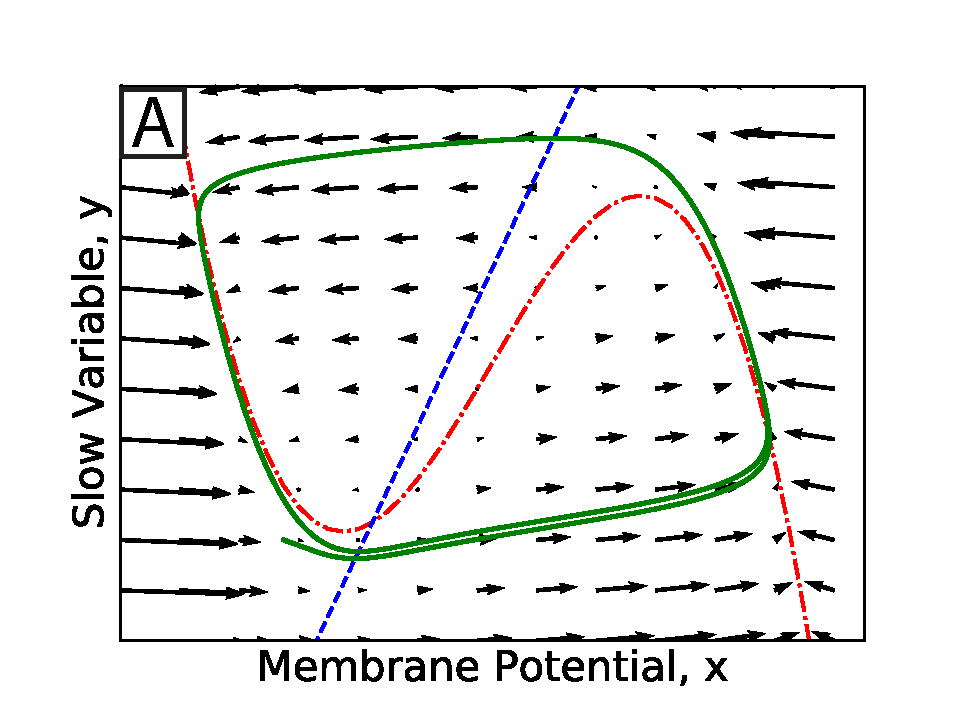
\includegraphics[width=0.47\columnwidth]{images/fn_vector_field.pdf}
  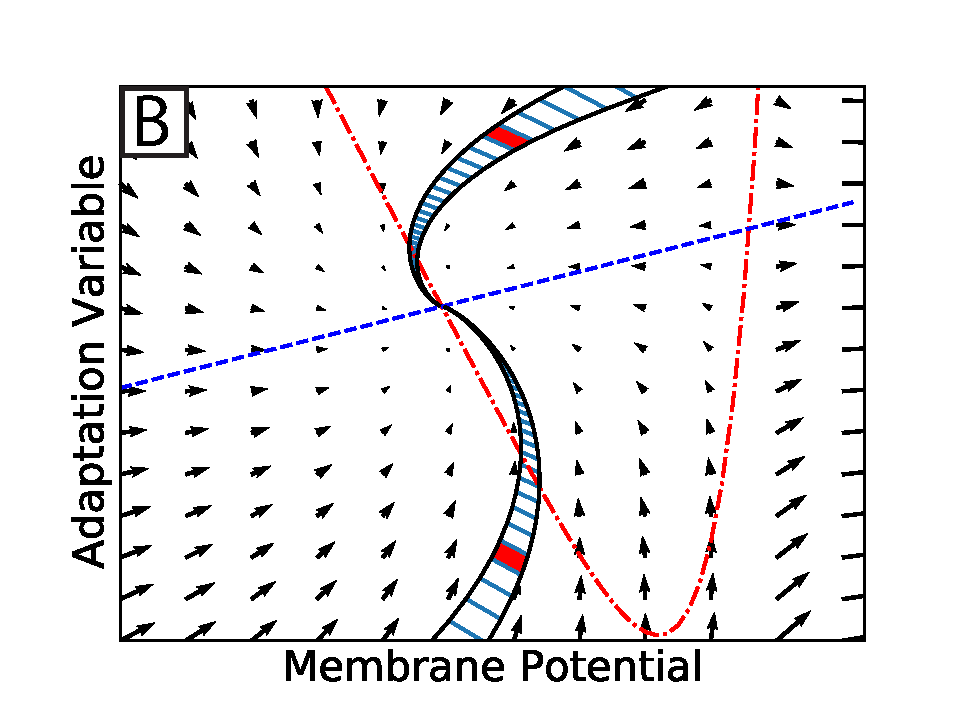
\includegraphics[width=0.47\columnwidth]{images/aexp_single_strip.pdf}
  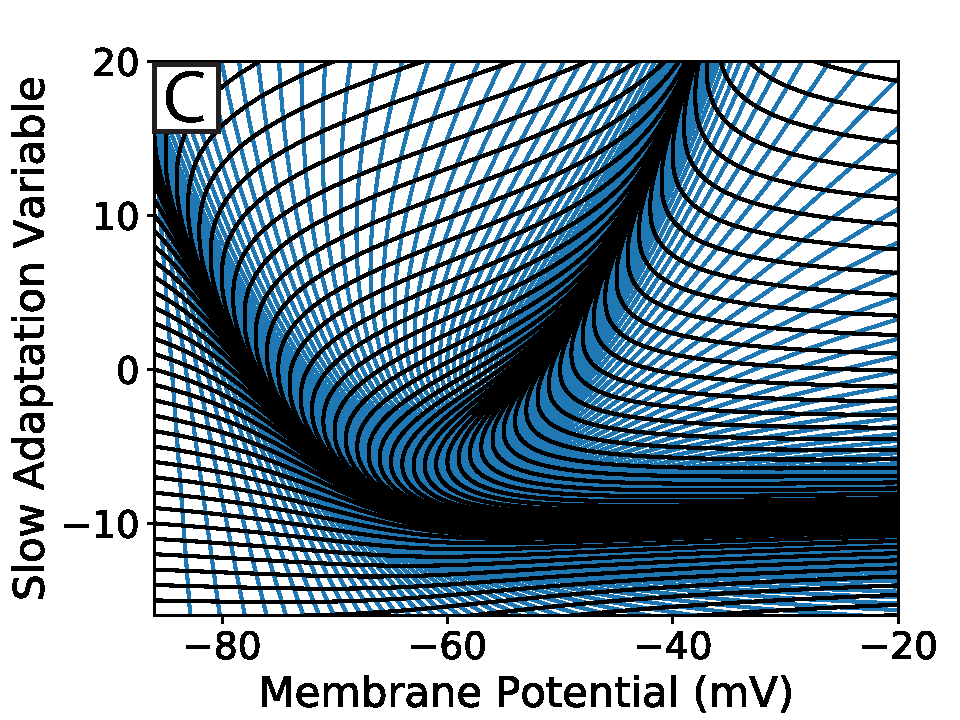
\includegraphics[width=0.45\columnwidth]{images/izh_mesh_empty.pdf}
  \caption{(A) A vector field of the FitzHugh-Nagumo neuron model \citep{fitzhugh1961impulses}. Arrows show the direction of motion of states through the field according to the dynamics of the model. The red broken dashed nullcline indicates where the change in x is zero. The blue dashed nullcline indicates where the change in y is zero. The green solid line shows a potential path (trajectory) of a neuron in the state space. (B) A vector field for the adaptive exponential integrate and fire neuron model \citep{brette2005}. Two strips are shown which follow the dynamics of the model and approach the stationary point where the nullclines cross. A strip is constructed between two trajectories in state space. Each time step of the two trajectories is used to segment the strip into cells. Because the strips approach a stationary point, they get thinner as the trajectories converge to the same point and cells get closer together as the distance in state space travelled reduces per time step (neurons slow down as they approach a stationary point). Per time step, probability mass is shifted from one cell to the next along the strip. (C) The state space of the Izhikevich simple neuron model \citep{izhikevich2003simple} which has been fully discretised into strips and cells.}
  \label{fig:strip}
\end{figure}

\begin{figure}[!htb]
  \centering
  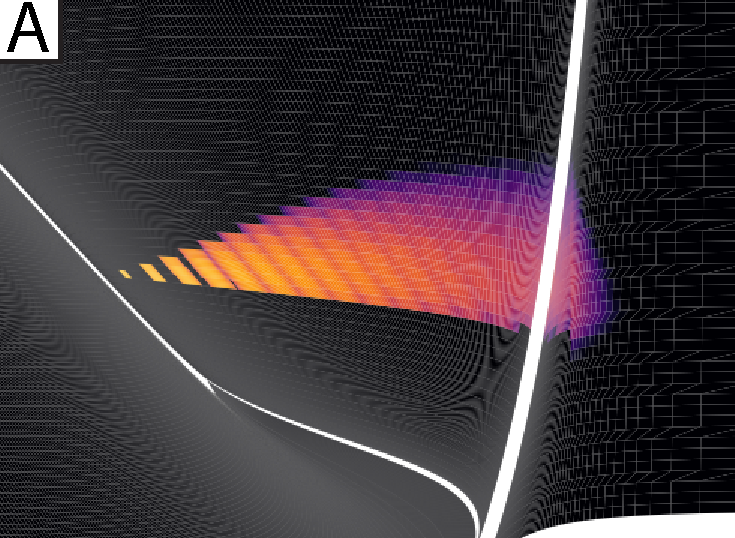
\includegraphics[width=0.45\columnwidth]{images/density_adex.pdf}
  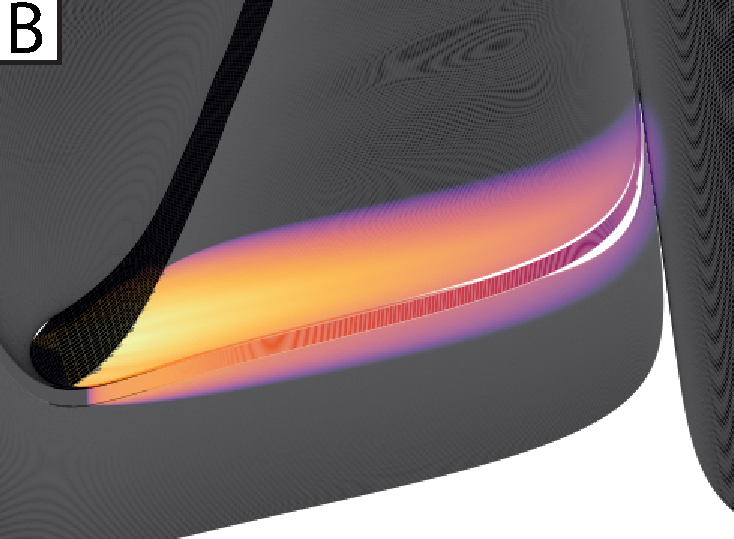
\includegraphics[width=0.45\columnwidth]{images/density_fn.pdf}
  \caption{Heat plots for the probability density functions of two populations in MIIND. Brightness (more yellow) indicates a higher probability mass. (A) When the Poisson master equation is solved, probability mass is pushed to the right (higher membrane potential) in discrete steps. As time passes, the discrete steps are smoothed out due to the movement of mass according to the deterministic dynamics (following the strip). (B) A combination of mass travelling along strips and being spread across the state space by noisy input produces the behaviour of the population.}
  \label{fig:desities}
\end{figure}

\begin{figure}[!htb]
  \centering
  \includegraphics[width=0.9\columnwidth]{images/neuroinformatics_reset_basic_image.png}
  \caption{For each time step, probability mass in the cells which lie across the threshold (threshold cells) is pushed onto the beginning of the refractory queue. There is one queue per threshold cell. During each subsequent time step, the mass is shifted one place along the queue until it reaches the penultimate place. A proportion of the mass, calculated according to the modulo of the refractory time and the time step, is transferred to the appropriate reset cell. The remaining mass is shifted to the final place in the queue. During the next time step, that remaining mass is transferred to the reset cell.}
  \label{fig:basicreset}
\end{figure}

\begin{figure}[!htb]
  \centering
  \includegraphics[width=\columnwidth]{images/reversal.png}
  \caption{Reversal mapping for a strip which approaches a stationary cell. The aim is to take probability mass from the end of the cell to the stationary cell. During MIIND's simulation loop, probability mass is first shifted one cell down the strip. The mass in the last cell is shifted to the first cell. The second step is for the reversal mapping to be applied. Therefore, the mapping should take mass from the first cell of the strip to the stationary cell.}
  \label{fig:reversal}
\end{figure}

\begin{figure}[!htb]
  \centering
  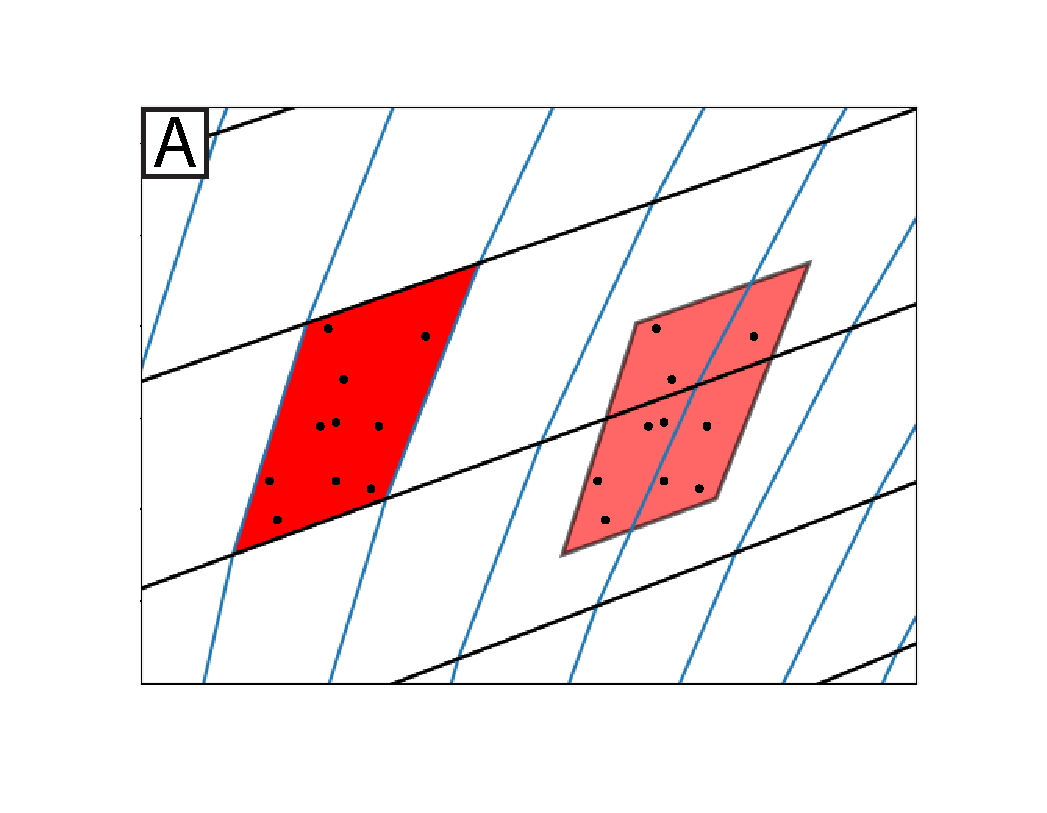
\includegraphics[width=0.45\columnwidth]{images/matrix_transition.pdf}
  \includegraphics[width=0.45\columnwidth]{images/lost.pdf}
  \caption{(A) To calculate the transitions of each cell due to a single incoming spike, the proportion of neurons that will end up in each target cell must be calculated. The Monte Carlo method of calculating the proportions is to take a number of points randomly placed in the source cell and translate them by the efficacy amount. The geometric solution is to translate the source cell vertices themselves and calculate the area overlap with target cells. (B) When using the Monte Carlo method, cells may be translated outside of the mesh but must be accounted for. The ``lost'' tool displays the missing points after \textbf{generate-matrix} has been called once. The user may then draw quadrilaterals (fiducial areas) around where the points lie. During the second call to \textbf{generate-matrix}, these areas will be used to search for nearby mesh cells to which the missing points can be attributed. }
  \label{fig:transitionlost}
\end{figure}

\begin{figure}[!htb]
  \centering
  \includegraphics[width=0.6\columnwidth]{images/mesh_issue_arrow.pdf}
  \caption{In MeshAlgorithm, when cells become shear, probability mass which is pushed to the right due to incoming spikes also moves laterally (downwards) because it is spread evenly across each cell.}
  \label{fig:meshissue}
\end{figure}

\begin{figure}[!htb]
  \centering
  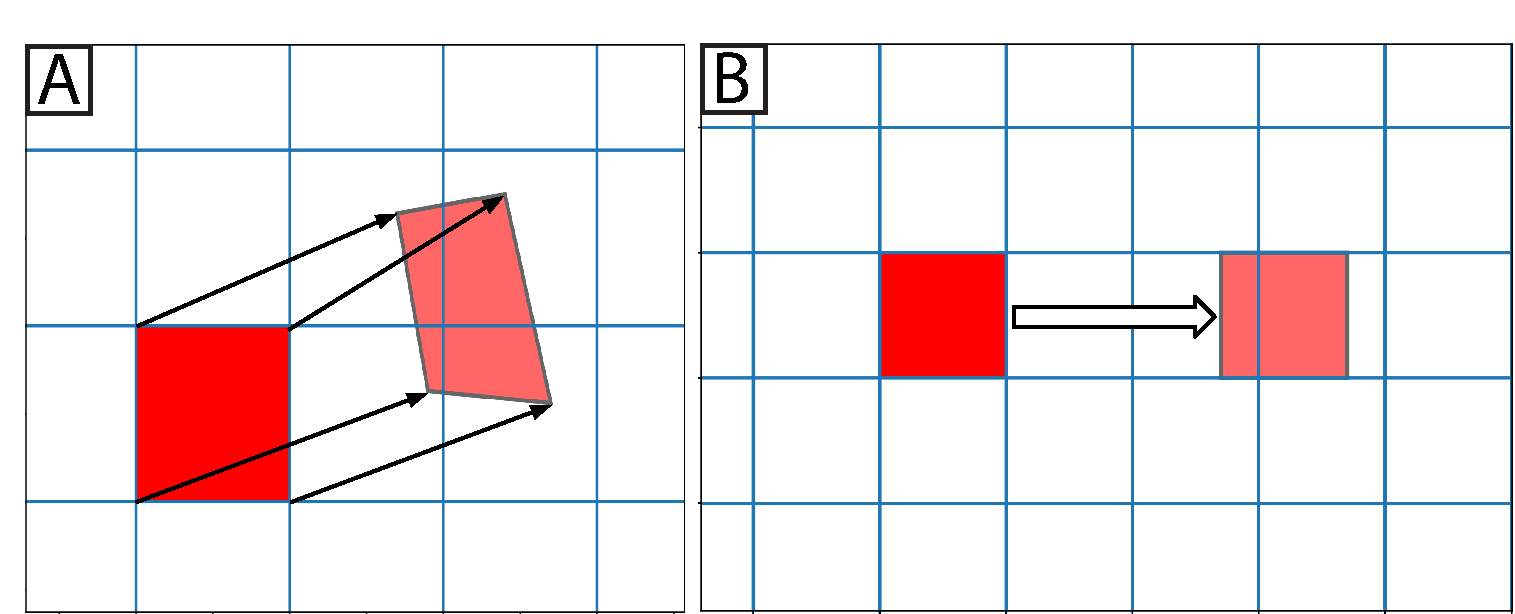
\includegraphics[width=\columnwidth]{images/grid_transitions.pdf}
  \caption{(A) The transition matrix for solving the deterministic dynamics of the population is generated by applying a single time step of the underlying neuron model to each vertex of each cell in the grid and calculating the proportion by area to each overlapping cell. (B) For a single incoming spike (with constant efficacy), all cells are translated by the same amount and therefore have the same resulting transition which can be used to solve the Poisson master equation. In fact, the transition will always involve at most two target cells and the proportions can be calculated knowing only the grid cell width and the efficacy.}
  \label{fig:grid}
\end{figure}

\begin{figure}[!htb]
  \centering
  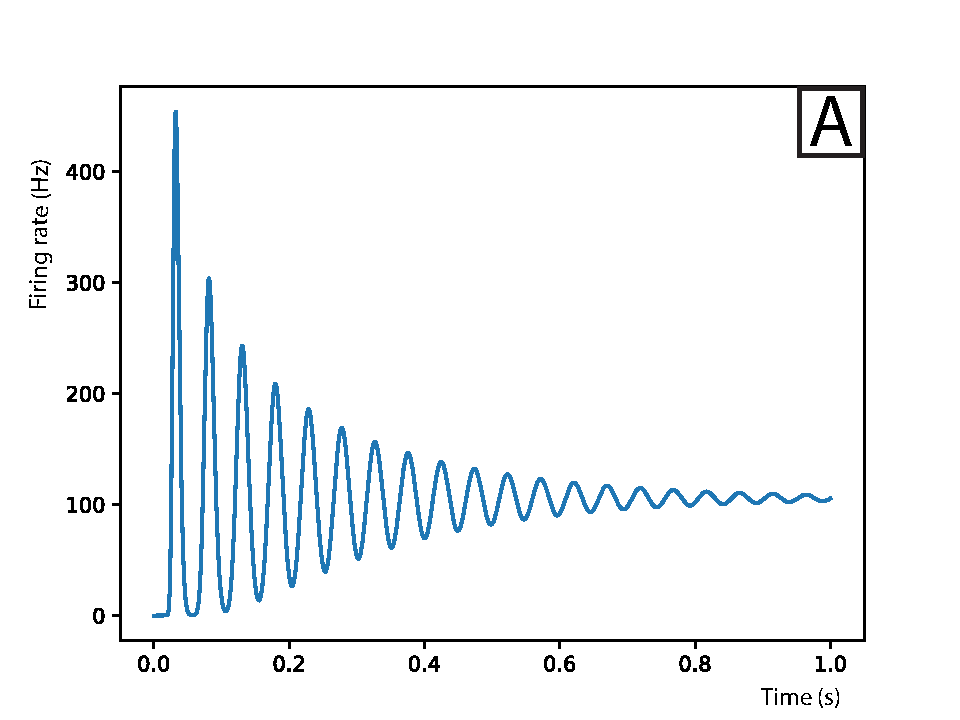
\includegraphics[width=0.45\columnwidth]{images/izh_rate.pdf}
  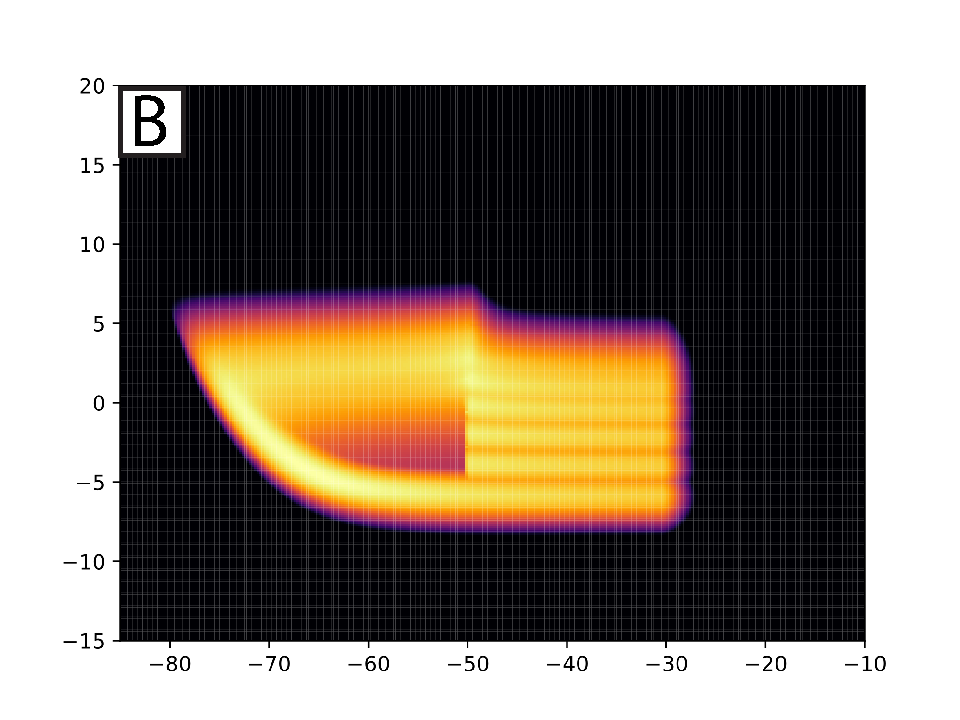
\includegraphics[width=0.45\columnwidth]{images/izh_density.pdf}
  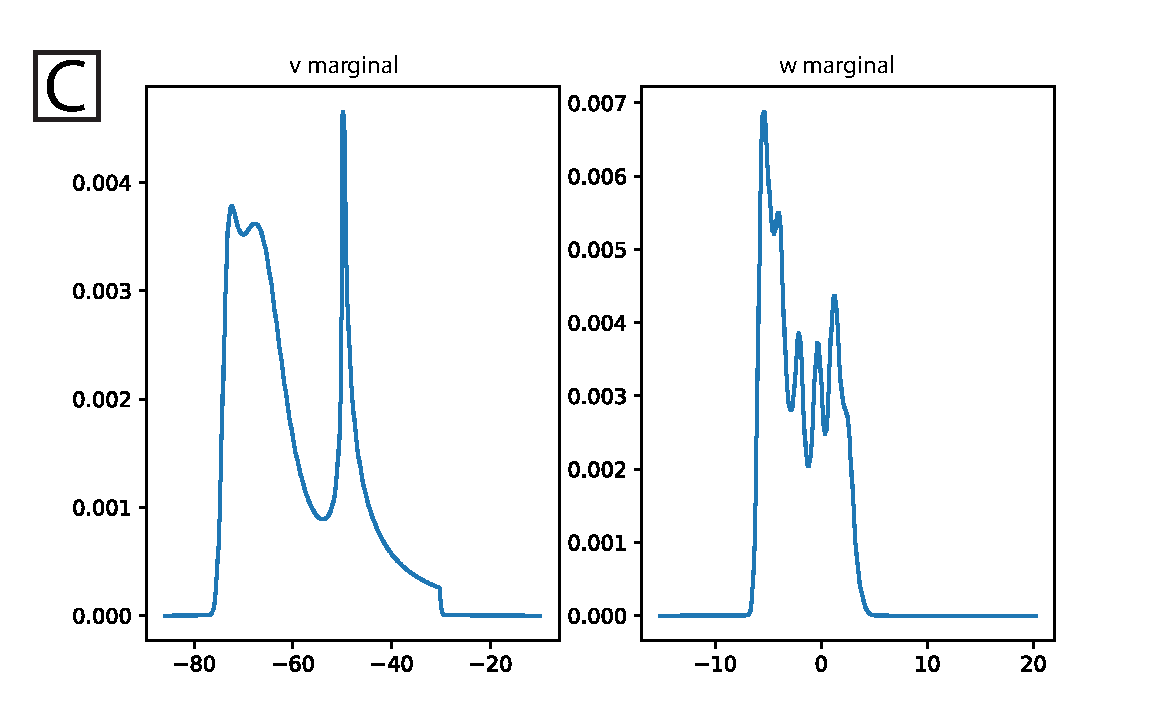
\includegraphics[width=0.6\columnwidth]{images/izh_marginal.pdf}
  \caption{(A) The average firing rate of the BURSTER population produced by calling the \textbf{rate} command. (B) A density plot of the BURSTER population produced by calling the \textbf{plot-density} command. (C) The marginal density plots produced by calling the \textbf{plot-marginals} command. }
\label{fig:rate_density_marginal}  
\end{figure}

\begin{figure}[!htb]
  \centering
  \includegraphics[width=0.45\columnwidth]{images/hindmarsh-rose.png}
  \caption{A density plot of a population of Hindmarsh-Rose neurons. The density is contained in a three dimensional volume such that each axis represents one of the time-dependent variables of the model. The volume has been rendered from a rotated and elevated position to more easily visualise the density.}
  \label{fig:hindmarshrose}
\end{figure}

%%% If you are submitting a figure with subfigures please combine these into one image file with part labels integrated.
%%% If you don't add the figures in the LaTeX files, please upload them when submitting the article.
%%% Frontiers will add the figures at the end of the provisional pdf automatically
%%% The use of LaTeX coding to draw Diagrams/Figures/Structures should be avoided. They should be external callouts including graphics.

\end{document}
